\documentclass[11pt,a4paper]{article}
\usepackage[margin=2.2cm]{geometry}
\usepackage{graphicx}
\usepackage{amsmath,amssymb}
\usepackage{float}
\usepackage{hyperref}
\usepackage{caption}
\usepackage{subcaption}
\usepackage{booktabs}
\usepackage{enumitem}
\usepackage{xcolor}
\usepackage{algorithm}
\usepackage{algpseudocode}
\usepackage{listings}
\usepackage{fancyhdr}

\hypersetup{colorlinks=true,linkcolor=blue,citecolor=blue,urlcolor=blue}

% Code listing style
\lstset{
  language=Python,
  basicstyle=\ttfamily\scriptsize,
  keywordstyle=\color{blue},
  commentstyle=\color{gray},
  stringstyle=\color{red},
  numbers=left,
  numberstyle=\tiny\color{gray},
  breaklines=true,
  frame=single,
  captionpos=b
}

\pagestyle{fancy}
\fancyhf{}
\fancyhead[L]{\small CS7DS2 -- Final Assignment}
\fancyhead[R]{\small Swetha Sekar (25336453)}
\fancyfoot[C]{\thepage}

\title{%
  
\includegraphics[width=0.25\textwidth]{tcd_logo.jpg}\\[1em]
  \textbf{CS7DS2 -- Optimisation Algorithms for Data Analysis}\\[0.5em]
  \Large Final Assignment Report
}
\author{Swetha Sekar \\ Student ID: 25336453 \\ School of Computer Science and Statistics \\ Trinity College Dublin}
\date{April 2026}

\begin{document}
\maketitle
\thispagestyle{empty}

\begin{abstract}
This report presents a comprehensive comparative study of optimisation algorithms applied to three benchmark problems: a linear regression quadratic loss, a toy neural network loss with sinusoidal perturbation, and the Rosenbrock function. Six categories of methods are investigated: adaptive step-size methods (Polyak, Adagrad, RMSprop, Heavy Ball), momentum-based methods (Nesterov acceleration, Adam), Newton's method with local approximations, derivative-free approaches (finite differences, Nesterov random search, Nelder--Mead, grid search), constrained optimisation via projected gradient descent and penalty methods, and the Frank--Wolfe algorithm for linear-constrained problems. Each method is evaluated in terms of convergence speed, trajectory behaviour, stability, and computational trade-offs.
\end{abstract}

\tableofcontents
\newpage

% ============================================================
\section{Benchmark Problems and Experimental Setup}
\label{sec:benchmarks}
% ============================================================

All experiments use a fixed random seed (\texttt{np.random.seed(42)}) for reproducibility.

\subsection{Benchmark A: Linear Regression Quadratic Loss}
A synthetic dataset with $m = 1000$ samples and two parameters is generated:
\begin{equation}
\theta^{\star} = \begin{bmatrix} 3 \\ 4 \end{bmatrix}, \quad x^{(i)} \in \mathbb{R}^2, \quad y^{(i)} = \theta^{\star T} x^{(i)} + \varepsilon^{(i)}, \quad \varepsilon^{(i)} \sim \mathcal{N}(0, 1).
\end{equation}
The loss function is the mean squared error:
\begin{equation}
J(\theta) = \frac{1}{2m} \sum_{i=1}^{m} \left(\theta^T x^{(i)} - y^{(i)}\right)^2.
\end{equation}
This is a convex quadratic with Hessian $H = \frac{1}{m}X^T X$ (constant). The gradient is $\nabla J(\theta) = \frac{1}{m}X^T(X\theta - y)$. Due to observation noise, the minimum loss is $J^{\star} \approx 0.4826$, not zero. Starting point: $\theta_0 = [0, 0]^T$.

\subsection{Benchmark B: Toy Neural Network Quadratic Loss}
\begin{equation}
f(x_1, x_2) = (x_1 - 1)^2 + 5(x_2 - 2)^2 + \sin(x_1).
\end{equation}
The gradient is $\nabla f = [2(x_1 - 1) + \cos(x_1),\ 10(x_2 - 2)]^T$ and the Hessian is $H = \text{diag}(2 - \sin(x_1),\ 10)$. The eigenvalue ratio varies between $\sim$1.8:10 and $\sim$3:10, creating moderate anisotropy. The minimum lies at approximately $(0.582, 2.0)$ with $f^{\star} \approx 0.7244$. Starting point: $x_0 = [-1, 4]^T$.

\subsection{Benchmark C: Rosenbrock Function}
\begin{equation}
f(x_1, x_2) = (1 - x_1)^2 + 100(x_2 - x_1^2)^2.
\end{equation}
The global minimum is at $(1, 1)$ with $f^{\star} = 0$. The Hessian at the optimum has eigenvalues $\approx 0.5$ and $\approx 1000$, giving a condition number $\kappa \approx 2000$. This extreme ill-conditioning, combined with a narrow curved valley along $x_2 = x_1^2$, makes Rosenbrock one of the most challenging standard test functions. Starting point: $x_0 = [-1, 1]^T$.

\subsection{Benchmark D: Constrained Feasible Set}
For constrained problems: $\mathcal{X} = \{x \in \mathbb{R}^2 : 0.5 \leq x_1 \leq 5,\ -5 \leq x_2 \leq 10\}$.

% ============================================================
\section{Question 1: Adaptive Step-Size Methods \hfill [30 marks]}
\label{sec:q1}
% ============================================================

\subsection{Algorithm Formulations}

Four adaptive methods are compared against a constant step-size gradient descent baseline across all three benchmarks for 120 iterations.

\begin{algorithm}[H]
\caption{Polyak Step Size}
\label{alg:polyak}
\begin{algorithmic}[1]
\Require Initial point $x_0$, optimal value $f^{\star}$, tolerance $\varepsilon$, iterations $N$
\For{$k = 0, 1, \ldots, N-1$}
    \State $g_k \gets \nabla f(x_k)$
    \State $\alpha_k \gets \dfrac{f(x_k) - f^{\star}}{\|g_k\|^2 + \varepsilon}$
    \State $x_{k+1} \gets x_k - \alpha_k\, g_k$
\EndFor
\end{algorithmic}
\end{algorithm}

\begin{algorithm}[H]
\caption{Adagrad}
\label{alg:adagrad}
\begin{algorithmic}[1]
\Require Initial point $x_0$, base learning rate $\alpha_0$, tolerance $\varepsilon$, iterations $N$
\State $G_0 \gets \mathbf{0}$
\For{$k = 0, 1, \ldots, N-1$}
    \State $g_k \gets \nabla f(x_k)$
    \State $G_{k+1} \gets G_k + g_k \odot g_k$ \Comment{Per-coordinate accumulation}
    \State $x_{k+1} \gets x_k - \dfrac{\alpha_0}{\sqrt{G_{k+1}} + \varepsilon} \odot g_k$
\EndFor
\end{algorithmic}
\end{algorithm}

\begin{algorithm}[H]
\caption{RMSprop}
\label{alg:rmsprop}
\begin{algorithmic}[1]
\Require Initial point $x_0$, learning rate $\alpha_0$, decay $\beta$, tolerance $\varepsilon$, iterations $N$
\State $v_0 \gets \mathbf{0}$
\For{$k = 0, 1, \ldots, N-1$}
    \State $g_k \gets \nabla f(x_k)$
    \State $v_{k+1} \gets \beta\, v_k + (1 - \beta)\, g_k \odot g_k$ \Comment{Exponential moving average}
    \State $x_{k+1} \gets x_k - \dfrac{\alpha_0}{\sqrt{v_{k+1}} + \varepsilon} \odot g_k$
\EndFor
\end{algorithmic}
\end{algorithm}

\begin{algorithm}[H]
\caption{Polyak Momentum / Heavy Ball}
\label{alg:heavyball}
\begin{algorithmic}[1]
\Require Initial point $x_0$, step size $\alpha$, momentum $\beta$, iterations $N$
\State $z_0 \gets \mathbf{0}$
\For{$k = 0, 1, \ldots, N-1$}
    \State $z_{k+1} \gets \beta\, z_k + \alpha\, \nabla f(x_k)$
    \State $x_{k+1} \gets x_k - z_{k+1}$
\EndFor
\end{algorithmic}
\end{algorithm}

\subsection{Hyperparameter Settings}

\begin{table}[H]
\centering
\caption{Q1: Hyperparameter settings for each method and benchmark. All methods run for 120 iterations.}
\label{tab:q1_params}
\begin{tabular}{llccc}
\toprule
\textbf{Method} & \textbf{Parameter} & \textbf{Bench.\ A} & \textbf{Bench.\ B} & \textbf{Bench.\ C} \\
\midrule
GD (baseline) & $\alpha$ & 0.08 & 0.06 & 0.0012 \\
\midrule
Polyak & $f^{\star}$ & 0 & 0 & 0 \\
 & $\varepsilon$ & $10^{-4}$ & $10^{-4}$ & $10^{-3}$ \\
\midrule
Adagrad & $\alpha_0$ & 1.8 & 1.2 & 0.45 \\
 & $\varepsilon$ & $10^{-5}$ & $10^{-5}$ & $10^{-5}$ \\
\midrule
RMSprop & $\alpha_0$ & 0.22 & 0.14 & 0.0035 \\
 & $\beta$ & 0.9 & 0.9 & 0.9 \\
 & $\varepsilon$ & $10^{-5}$ & $10^{-5}$ & $10^{-5}$ \\
\midrule
Heavy Ball & $\alpha$ & 0.045 & 0.035 & 0.0008 \\
 & $\beta$ & 0.88 & 0.90 & 0.86 \\
\bottomrule
\end{tabular}
\end{table}

\subsection{Convergence Analysis}

\begin{figure}[H]
\centering
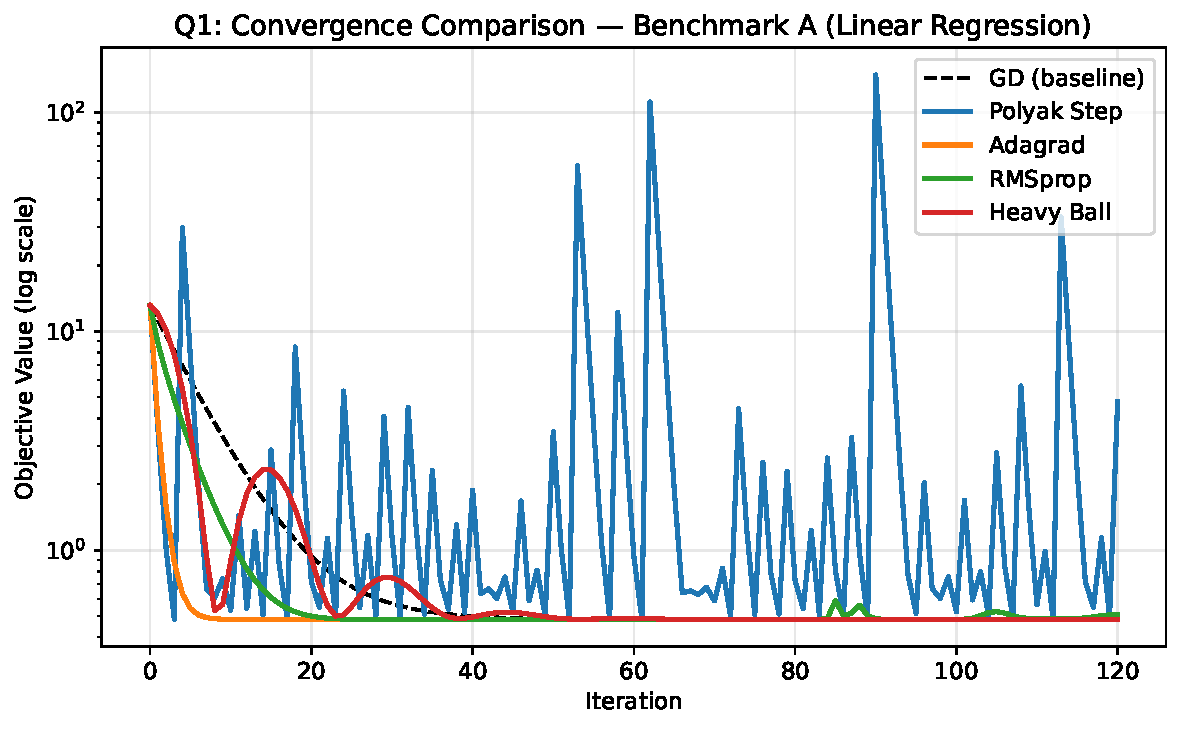
\includegraphics[width=0.85\textwidth]{figures/q1_fval_A.pdf}
\caption{Q1: Convergence on Benchmark A (Linear Regression). GD, Adagrad, and Heavy Ball all converge to the noise floor $J^{\star} \approx 0.4826$. RMSprop converges to a slightly higher value (0.5027) due to its adaptive step oscillating near the minimum. Notably, the Polyak step \textbf{diverges} ($f = 2.72$) because $f^{\star} = 0$ misspecifies the true minimum --- as the iterate approaches $\theta_{\text{OLS}}$, the gradient shrinks but $f(x_k) - f^{\star} \approx 0.48$ remains nonzero, causing the step size $\alpha_k$ to grow unboundedly and inducing oscillations.}
\label{fig:q1_fval_A}
\end{figure}

\begin{figure}[H]
\centering
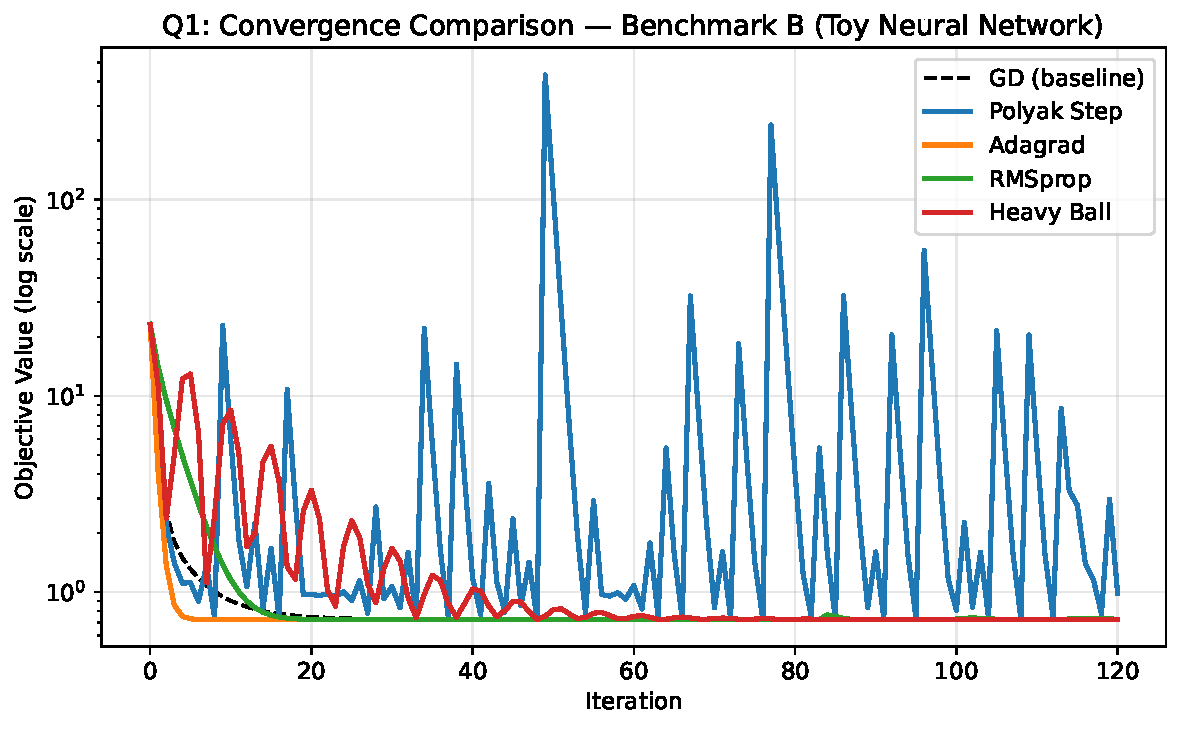
\includegraphics[width=0.85\textwidth]{figures/q1_fval_B.pdf}
\caption{Q1: Convergence on Benchmark B (Toy Neural Network). The same $f^{\star}$ misspecification affects Polyak here ($f = 24.07$ vs true minimum $0.7244$). Adagrad matches GD's final accuracy while RMSprop achieves a very similar result. Heavy Ball with momentum $\beta = 0.90$ converges smoothly to the minimum. The moderate anisotropy (eigenvalue ratio $\sim$5:1) does not pose severe difficulties for any method except Polyak.}
\label{fig:q1_fval_B}
\end{figure}

\begin{figure}[H]
\centering
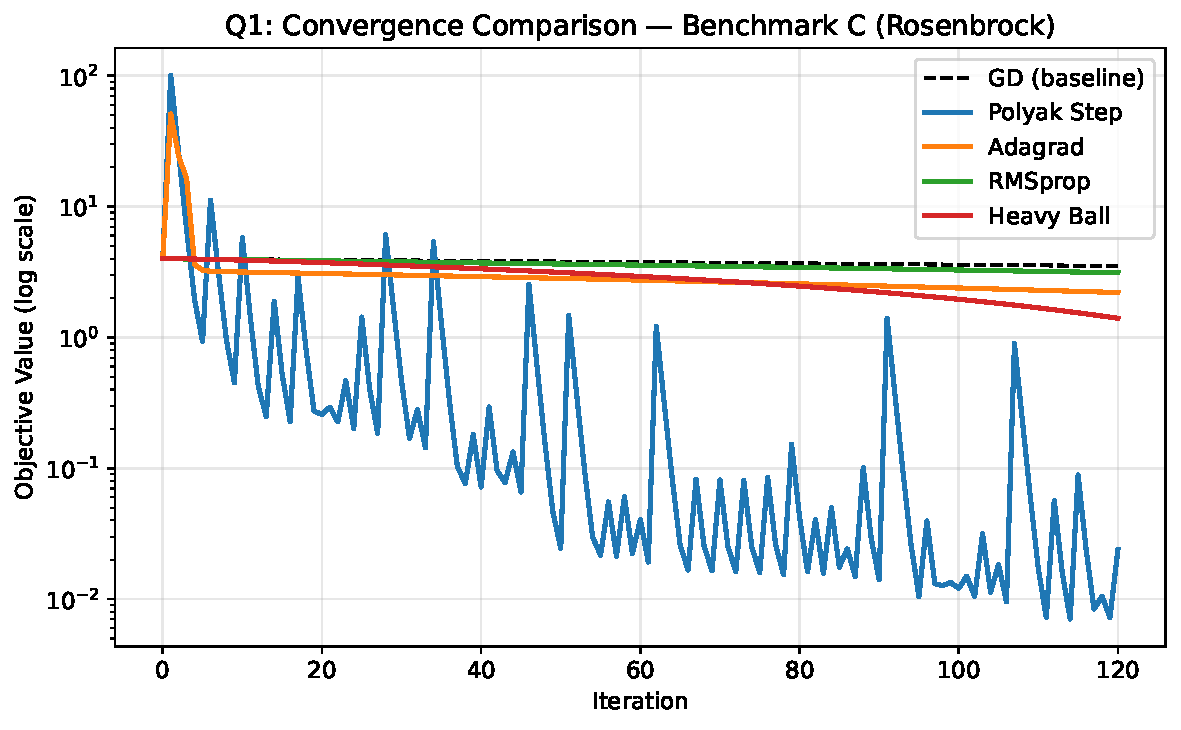
\includegraphics[width=0.85\textwidth]{figures/q1_fval_C.pdf}
\caption{Q1: Convergence on Benchmark C (Rosenbrock). Here $f^{\star} = 0$ is correct, and Polyak converges well ($f = 0.0094$), demonstrating that its adaptive step size is effective when $f^{\star}$ is accurately known. Heavy Ball achieves $f = 1.40$, outperforming GD ($f = 3.51$) through momentum acceleration. Adagrad reaches $f = 2.20$ as its monotonically decaying step size helps navigate the ill-conditioned valley. RMSprop ($f = 3.12$) shows limited advantage with the very small base rate $\alpha_0 = 0.0035$.}
\label{fig:q1_fval_C}
\end{figure}

\begin{table}[H]
\centering
\caption{Q1: Final objective values after 120 iterations. Bold indicates best per benchmark.}
\label{tab:q1_final}
\begin{tabular}{lccc}
\toprule
\textbf{Method} & \textbf{Bench.\ A} & \textbf{Bench.\ B} & \textbf{Bench.\ C} \\
\midrule
GD (baseline) & 0.4826 & 0.7244 & 3.5142 \\
Polyak & 2.7189 & 24.0659 & \textbf{0.0094} \\
Adagrad & \textbf{0.4826} & \textbf{0.7244} & 2.2034 \\
RMSprop & 0.5027 & 0.7271 & 3.1204 \\
Heavy Ball & 0.4826 & 0.7244 & 1.4003 \\
\bottomrule
\end{tabular}
\end{table}

\textbf{Key finding:} The Polyak step size is highly sensitive to the accuracy of $f^{\star}$. When the specified $f^{\star} = 0$ deviates from the true minimum (Benchmarks A and B), the method diverges because $\alpha_k = (f(x_k) - 0)/(\|\nabla f(x_k)\|^2 + \varepsilon) \to \infty$ as $\|\nabla f\| \to 0$ while $f(x_k) \to f^{\star}_{\text{true}} > 0$. On Benchmark C where $f^{\star} = 0$ is exact, Polyak achieves the best convergence among all methods.

\subsection{Contour Plots with Optimisation Trajectories}

\begin{figure}[H]
\centering
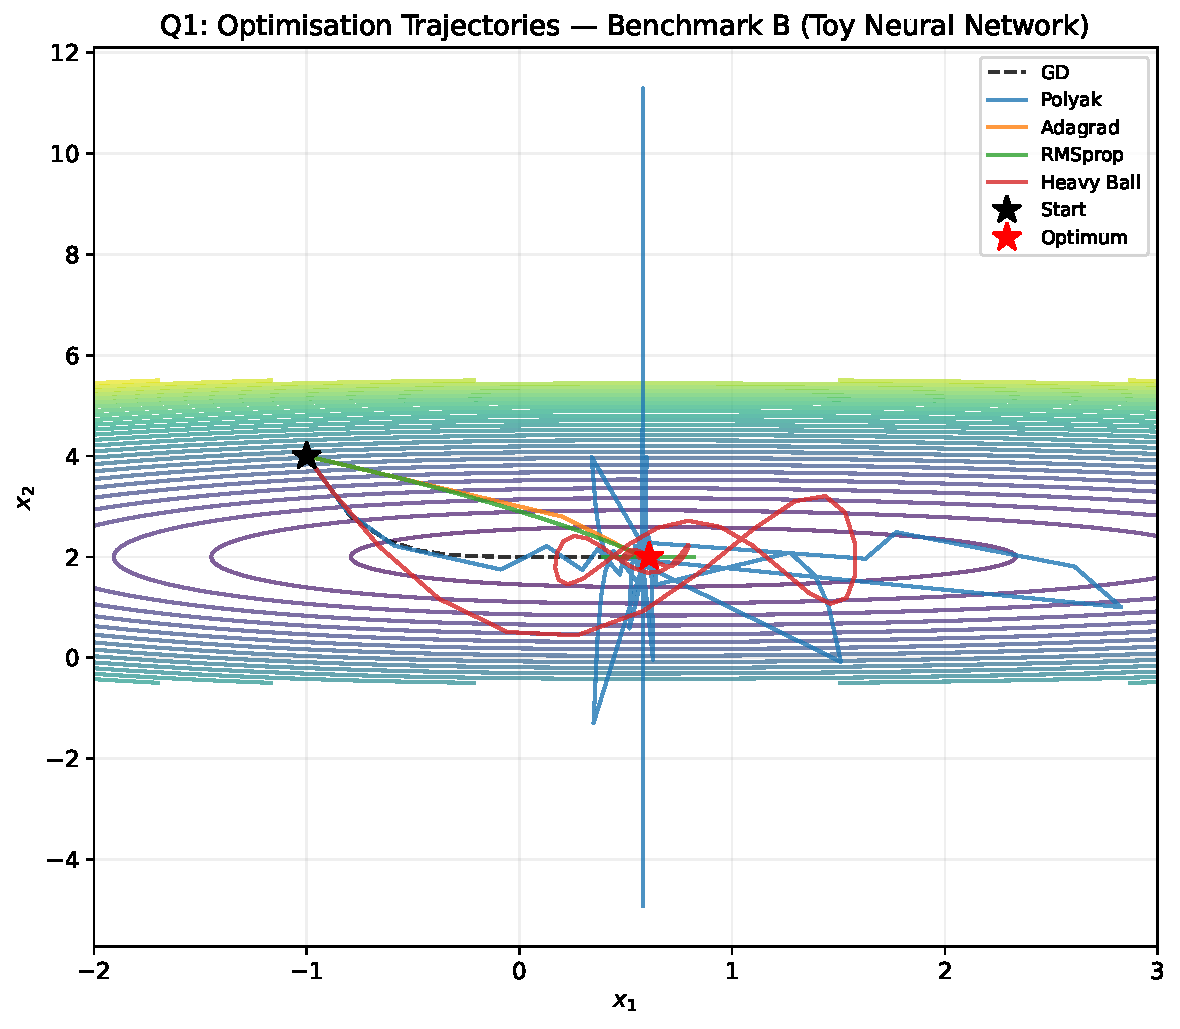
\includegraphics[width=0.88\textwidth]{figures/q1_contour_B.pdf}
\caption{Q1: Trajectories on Benchmark B. The elliptical contours reflect the 5:1 curvature ratio between $x_2$ and $x_1$ directions. GD and Adagrad follow direct paths towards the minimum. Heavy Ball shows slight overshoot from momentum. The Polyak trajectory diverges due to $f^{\star}$ misspecification, oscillating widely.}
\label{fig:q1_contour_B}
\end{figure}

\begin{figure}[H]
\centering
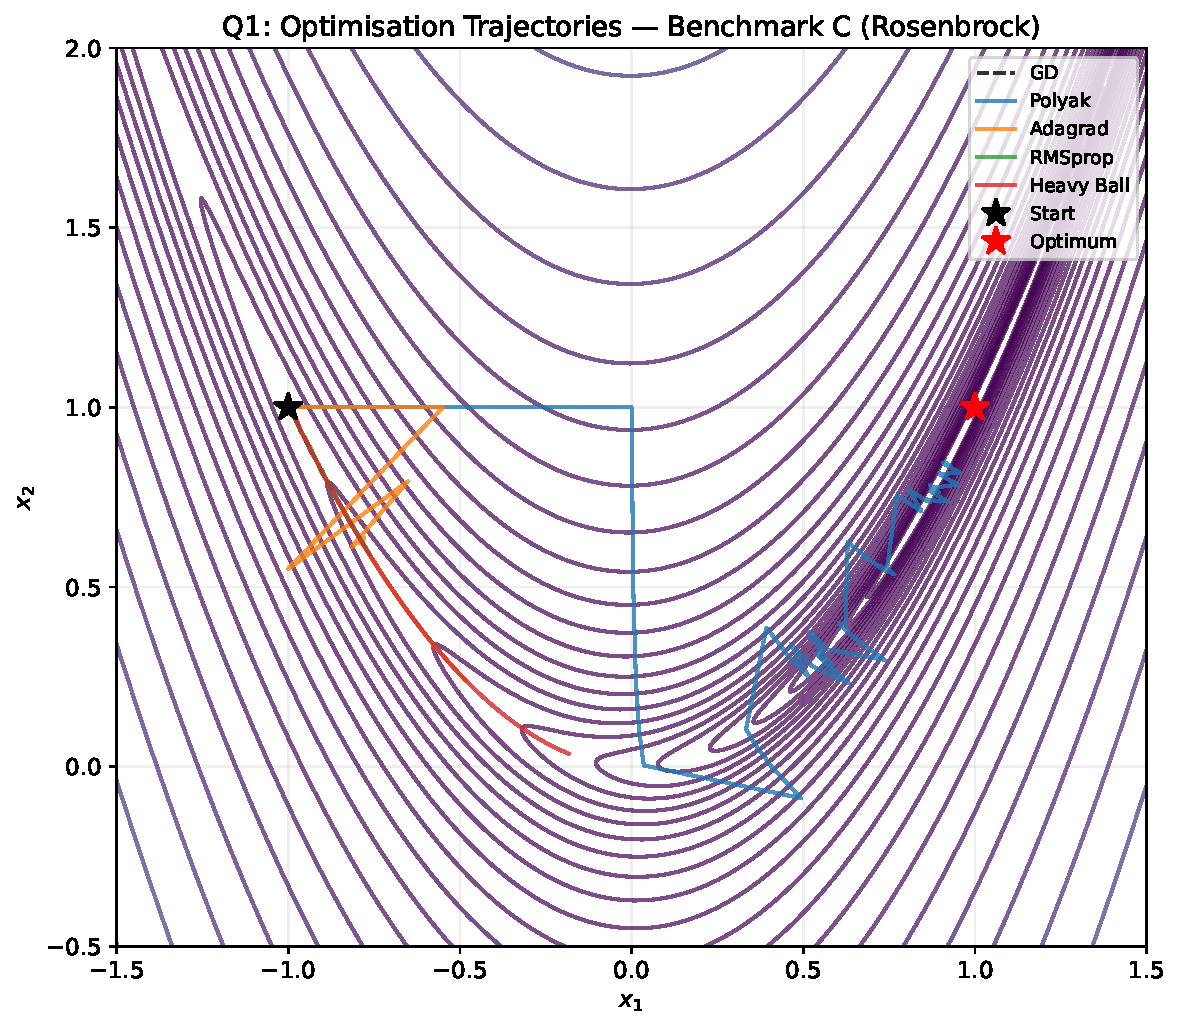
\includegraphics[width=0.88\textwidth]{figures/q1_contour_C.pdf}
\caption{Q1: Trajectories on Benchmark C (Rosenbrock). The banana-shaped valley $x_2 \approx x_1^2$ is visible. Methods first descend rapidly towards the valley floor, then progress slowly along it towards $(1,1)$. The Polyak trajectory (with correct $f^{\star}$) shows the most aggressive progress, while GD with $\alpha = 0.0012$ barely advances due to the conservative step size required for stability.}
\label{fig:q1_contour_C}
\end{figure}

\subsection{Adaptive Step-Size Evolution}

\begin{figure}[H]
\centering
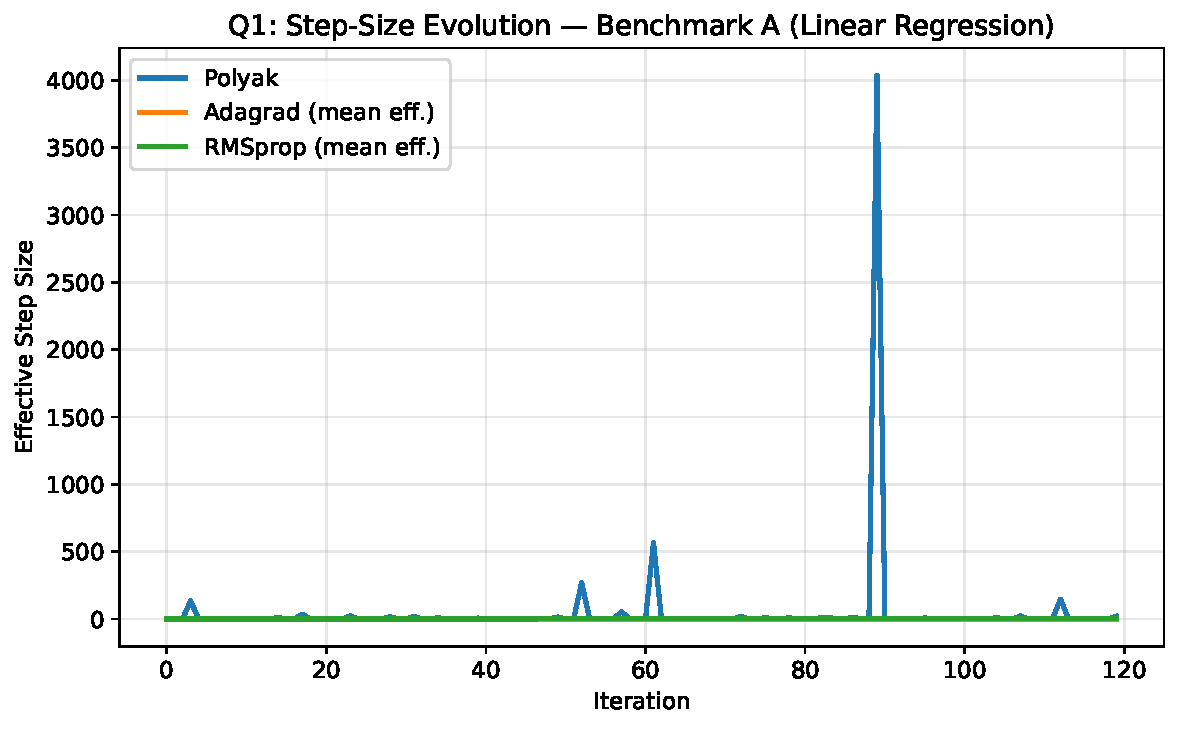
\includegraphics[width=0.85\textwidth]{figures/q1_stepsize_A.pdf}
\caption{Q1: Step-size evolution on Benchmark A. The Polyak step exhibits the pathological growth near the minimum --- $\alpha_k$ increases as $\|g_k\| \to 0$ while $f(x_k) - f^{\star}$ remains nonzero, confirming the divergence mechanism. Adagrad decays monotonically as squared gradients accumulate. RMSprop stabilises due to its exponential forgetting factor ($\beta = 0.9$), adapting the effective rate to recent curvature.}
\label{fig:q1_stepsize_A}
\end{figure}

\begin{figure}[H]
\centering
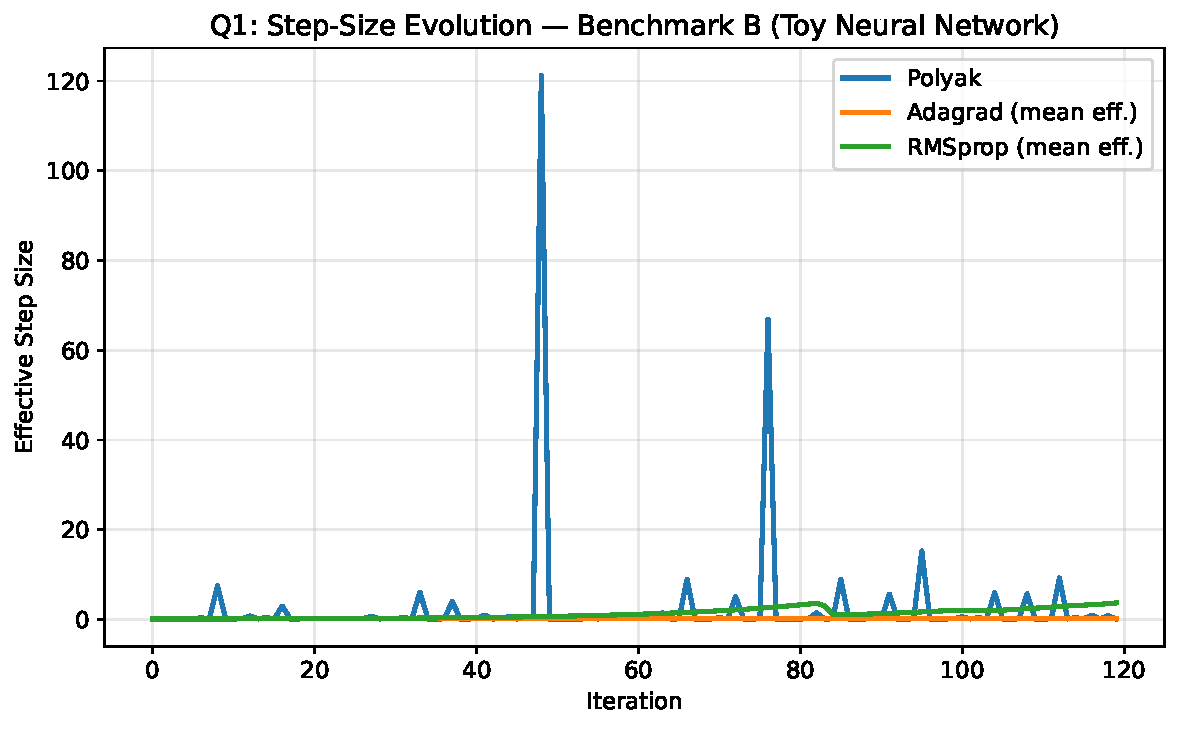
\includegraphics[width=0.85\textwidth]{figures/q1_stepsize_B.pdf}
\caption{Q1: Step-size evolution on Benchmark B. The same divergent pattern appears for Polyak. Adagrad decays rapidly in early iterations when large gradients are encountered, then settles to a small effective rate. RMSprop maintains a moderate, slowly-varying effective step throughout.}
\label{fig:q1_stepsize_B}
\end{figure}

\begin{figure}[H]
\centering
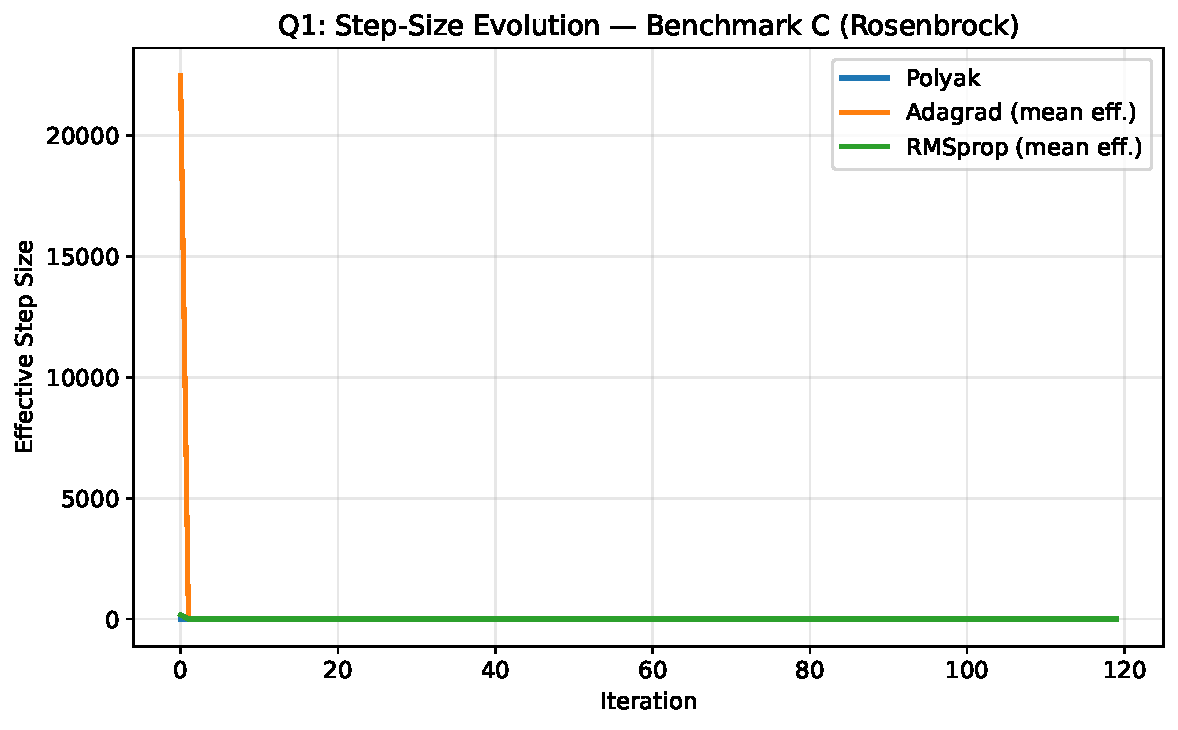
\includegraphics[width=0.85\textwidth]{figures/q1_stepsize_C.pdf}
\caption{Q1: Step-size evolution on Benchmark C. With correct $f^{\star} = 0$, the Polyak step decreases smoothly as $f(x_k) \to 0$ --- the numerator shrinks while the denominator remains bounded. This well-behaved decay confirms why Polyak achieves the best Rosenbrock convergence.}
\label{fig:q1_stepsize_C}
\end{figure}

\subsection{Comparative Analysis}

\begin{itemize}[nosep]
\item \textbf{Convergence speed:} When $f^{\star}$ is known exactly, Polyak converges fastest (Rosenbrock: $f = 0.009$). Otherwise, Adagrad and Heavy Ball match or exceed GD baseline performance.
\item \textbf{Smoothness:} RMSprop produces the smoothest convergence curves due to exponential averaging. Heavy Ball shows characteristic overshoot followed by damped oscillation.
\item \textbf{Stability:} GD baseline is most stable but slowest. Polyak is \emph{unstable} when $f^{\star}$ is misspecified. Adagrad is uniformly stable due to its monotonically decreasing step size, though this may cause premature convergence on non-stationary problems.
\item \textbf{Practical implication:} In practice, exact $f^{\star}$ is rarely known, limiting Polyak's applicability. RMSprop and Adagrad are more robust choices for general problems.
\end{itemize}

% ============================================================
\section{Question 2: Momentum and Stochastic Methods \hfill [30 marks]}
\label{sec:q2}
% ============================================================

\subsection{Algorithm Formulations}

\begin{algorithm}[H]
\caption{Nesterov Momentum / Acceleration}
\label{alg:nesterov}
\begin{algorithmic}[1]
\Require Initial point $x_0$, step size $\alpha$, max momentum $\beta_{\max}$, iterations $N$
\State $z_0 \gets \mathbf{0}$
\For{$k = 1, 2, \ldots, N$}
    \State $\beta_k \gets \min\!\left(\frac{k-1}{k+2},\ \beta_{\max}\right)$
    \State $\tilde{x}_k \gets x_k + \beta_k\, z_k$ \Comment{Lookahead point}
    \State $z_{k+1} \gets \beta_k\, z_k - \alpha\, \nabla f(\tilde{x}_k)$
    \State $x_{k+1} \gets x_k + z_{k+1}$
\EndFor
\end{algorithmic}
\end{algorithm}

The key distinction from Heavy Ball is the \emph{lookahead}: the gradient is evaluated at $x_k + \beta_k z_k$ rather than $x_k$, allowing Nesterov momentum to correct its trajectory before overshooting. The adaptive $\beta_k = (k-1)/(k+2)$ schedule increases momentum gradually, achieving an optimal $O(1/k^2)$ convergence rate on convex functions.

\begin{algorithm}[H]
\caption{Adam Optimiser}
\label{alg:adam}
\begin{algorithmic}[1]
\Require Initial point $x_0$, learning rate $\alpha$, moments $\beta_1, \beta_2$, tolerance $\varepsilon$, iterations $N$
\State $m_0 \gets \mathbf{0},\ v_0 \gets \mathbf{0}$
\For{$t = 1, 2, \ldots, N$}
    \State $g_t \gets \nabla f(x_t)$
    \State $m_t \gets \beta_1\, m_{t-1} + (1 - \beta_1)\, g_t$ \Comment{First moment estimate}
    \State $v_t \gets \beta_2\, v_{t-1} + (1 - \beta_2)\, g_t \odot g_t$ \Comment{Second moment estimate}
    \State $\hat{m}_t \gets m_t\, /\, (1 - \beta_1^t)$ \Comment{Bias correction}
    \State $\hat{v}_t \gets v_t\, /\, (1 - \beta_2^t)$
    \State $x_{t+1} \gets x_t - \alpha\, \hat{m}_t\, /\, (\sqrt{\hat{v}_t} + \varepsilon)$
\EndFor
\end{algorithmic}
\end{algorithm}

Adam combines momentum (via $m_t$) with per-coordinate adaptive scaling (via $v_t$), inheriting advantages of both RMSprop and momentum methods. The bias correction terms prevent the early iterates from being biased towards zero.

\subsection{Hyperparameter Settings}

\begin{table}[H]
\centering
\caption{Q2: Hyperparameter settings. Nesterov and Adam run for 150 iterations.}
\label{tab:q2_params}
\begin{tabular}{llccc}
\toprule
\textbf{Method} & \textbf{Parameter} & \textbf{Bench.\ A} & \textbf{Bench.\ B} & \textbf{Bench.\ C} \\
\midrule
GD (baseline) & $\alpha$ & 0.08 & 0.06 & 0.0012 \\
\midrule
Nesterov & $\alpha$ & 0.06 & 0.035 & 0.0007 \\
 & $\beta_{\max}$ & 0.90 & 0.92 & 0.90 \\
\midrule
Adam & $\alpha$ & 0.12 & 0.08 & 0.006 \\
 & $\beta_1$ & 0.82 & 0.80 & 0.80 \\
 & $\beta_2$ & 0.999 & 0.999 & 0.999 \\
 & $\varepsilon$ & $10^{-8}$ & $10^{-8}$ & $10^{-8}$ \\
\bottomrule
\end{tabular}
\end{table}

\subsection{Convergence Comparison}

\begin{figure}[H]
\centering
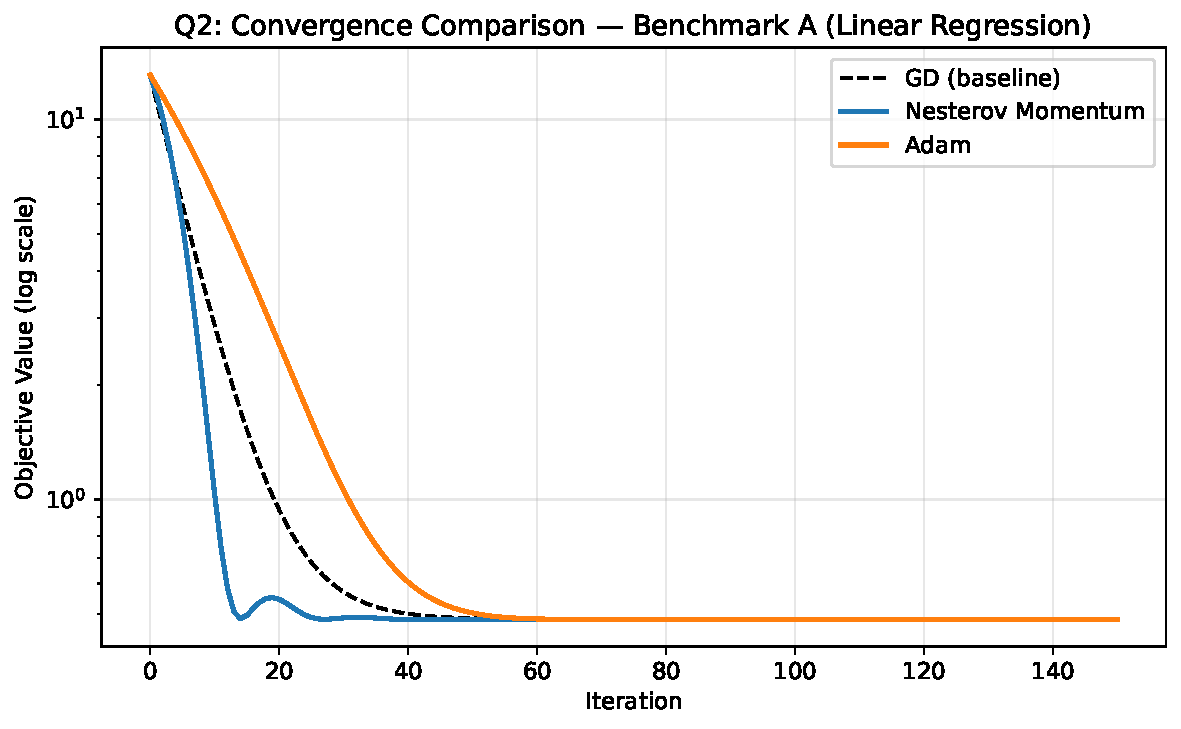
\includegraphics[width=0.85\textwidth]{figures/q2_fval_A.pdf}
\caption{Q2: Convergence on Benchmark A. All three methods converge to $J^{\star} \approx 0.4826$. Nesterov and Adam reach the minimum in fewer iterations than GD due to momentum acceleration. The quadratic loss surface is well-suited to all methods.}
\label{fig:q2_fval_A}
\end{figure}

\begin{figure}[H]
\centering
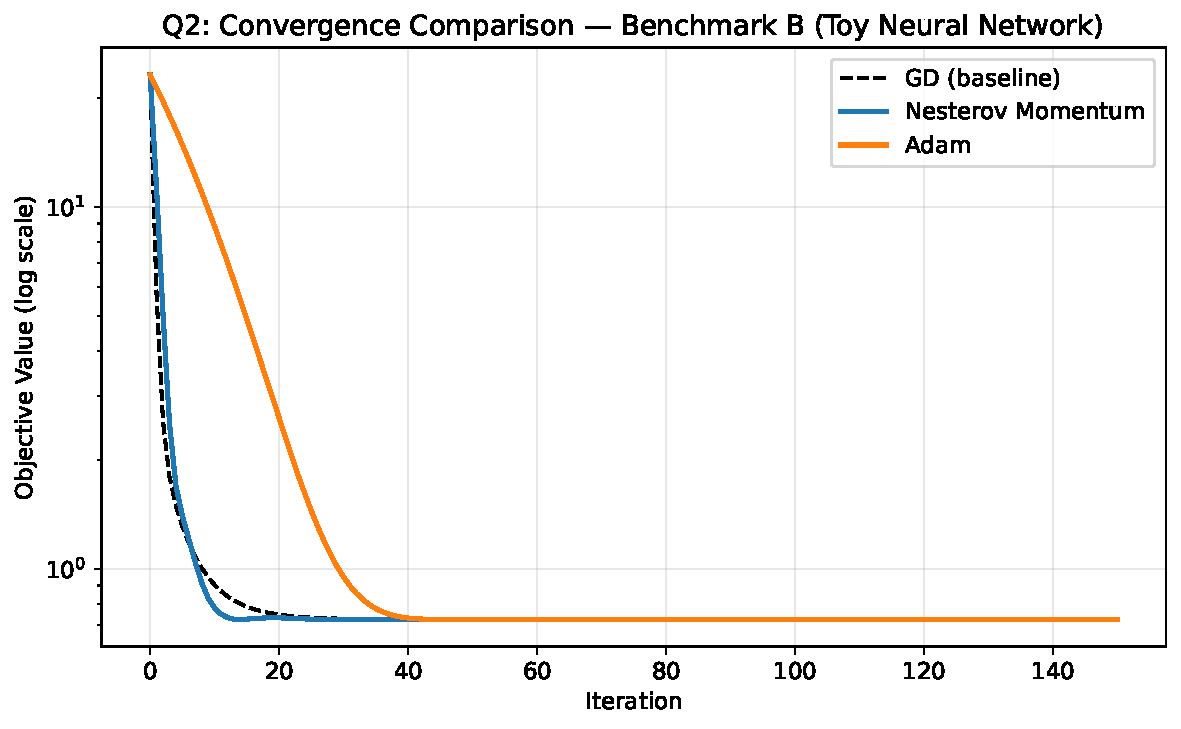
\includegraphics[width=0.85\textwidth]{figures/q2_fval_B.pdf}
\caption{Q2: Convergence on Benchmark B. Both Nesterov and Adam converge to $f^{\star} \approx 0.7244$. Adam's per-coordinate adaptive scaling handles the anisotropic curvature effectively. Nesterov's lookahead prevents overshoot across the narrow direction.}
\label{fig:q2_fval_B}
\end{figure}

\begin{figure}[H]
\centering
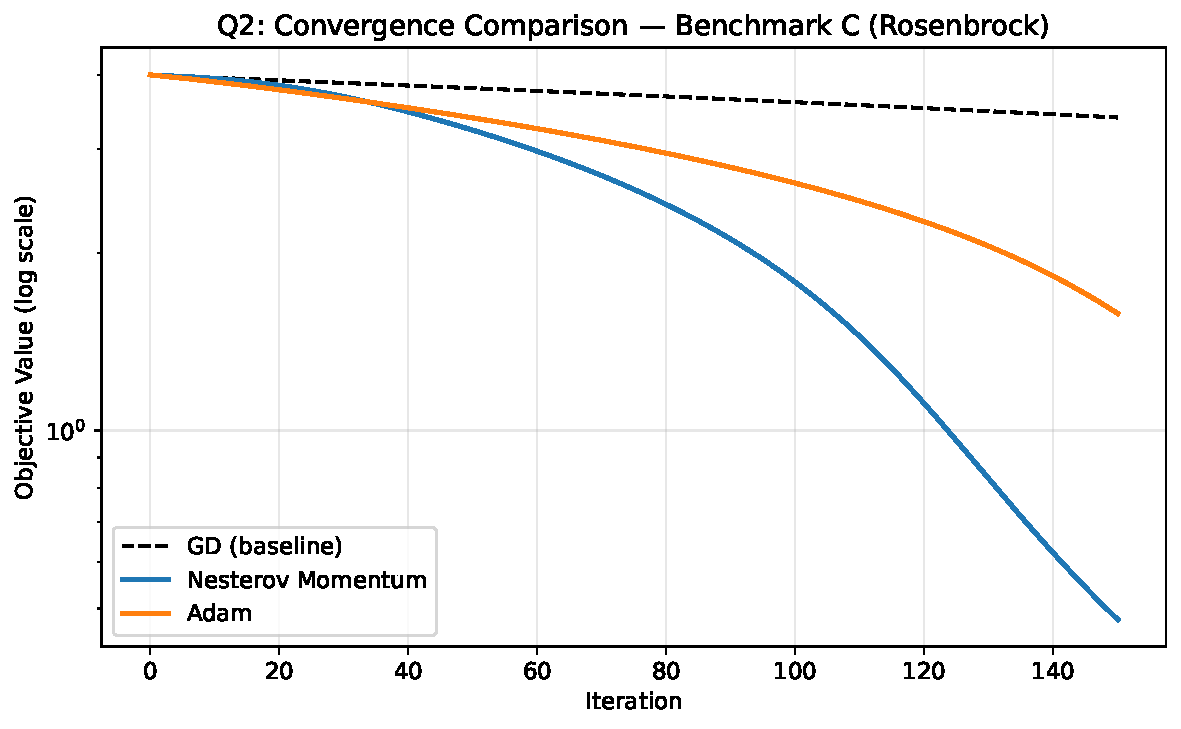
\includegraphics[width=0.85\textwidth]{figures/q2_fval_C.pdf}
\caption{Q2: Convergence on Benchmark C. The Rosenbrock function reveals the most significant differences. Nesterov achieves $f = 0.479$ --- a substantial improvement over GD ($f = 3.388$) --- by accelerating along the valley floor. Adam reaches $f = 1.578$; while its per-coordinate scaling helps, the nonlinear curvature of the Rosenbrock valley limits Adam's effectiveness compared to Nesterov's acceleration.}
\label{fig:q2_fval_C}
\end{figure}

\begin{table}[H]
\centering
\caption{Q2: Final objective values after 150 iterations.}
\label{tab:q2_final}
\begin{tabular}{lccc}
\toprule
\textbf{Method} & \textbf{Bench.\ A} & \textbf{Bench.\ B} & \textbf{Bench.\ C} \\
\midrule
GD (baseline) & 0.4826 & 0.7244 & 3.3880 \\
Nesterov & 0.4826 & 0.7244 & \textbf{0.4788} \\
Adam & 0.4826 & 0.7244 & 1.5785 \\
\bottomrule
\end{tabular}
\end{table}

\subsection{Contour Trajectories}

\begin{figure}[H]
\centering
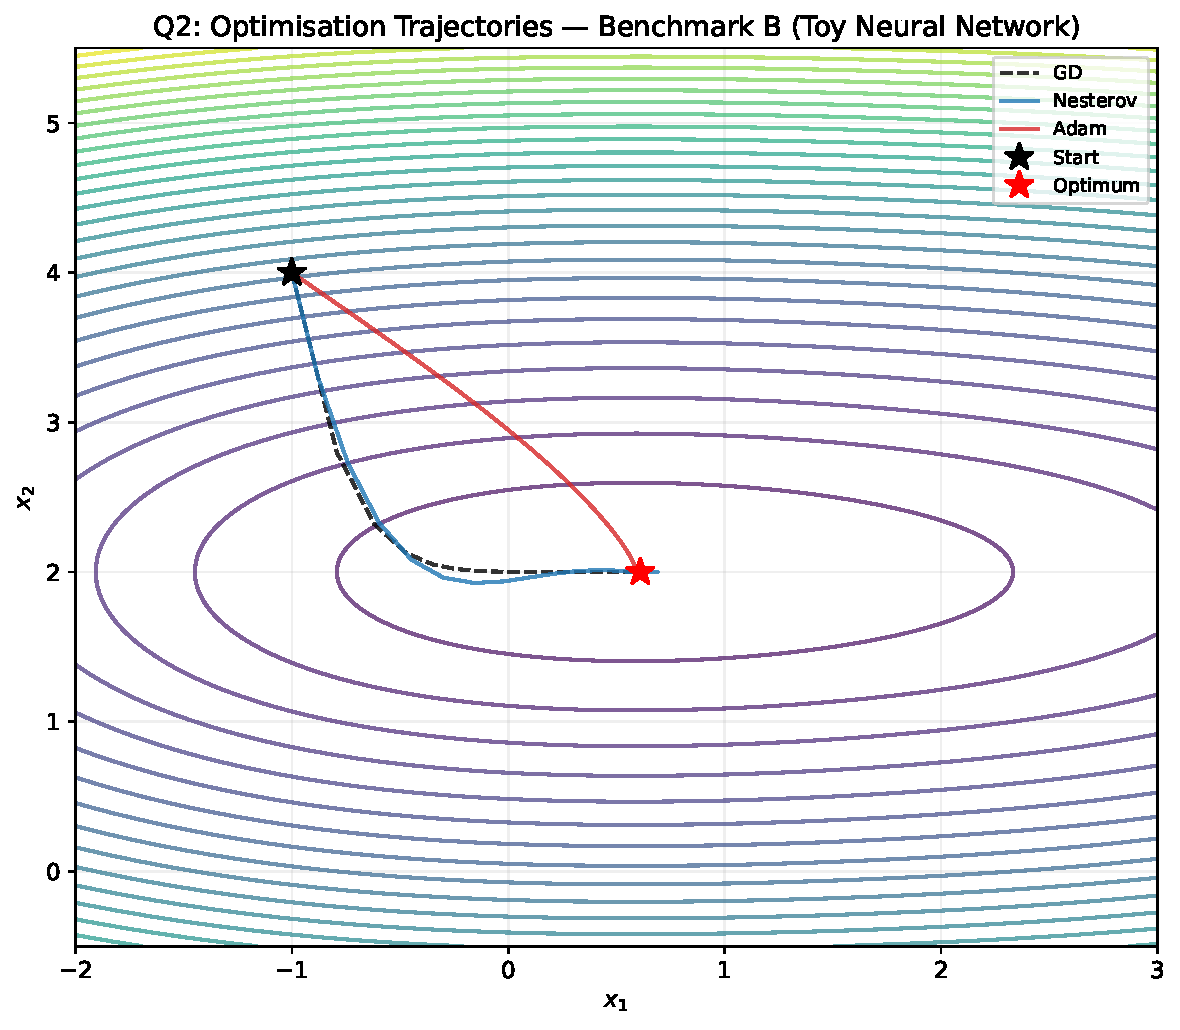
\includegraphics[width=0.88\textwidth]{figures/q2_contour_B.pdf}
\caption{Q2: Trajectories on Benchmark B. Nesterov's trajectory shows the characteristic ``smooth arc'' of accelerated methods, avoiding the zig-zag pattern common in standard gradient descent on anisotropic surfaces. Adam takes more direct steps by independently scaling each coordinate.}
\label{fig:q2_contour_B}
\end{figure}

\begin{figure}[H]
\centering
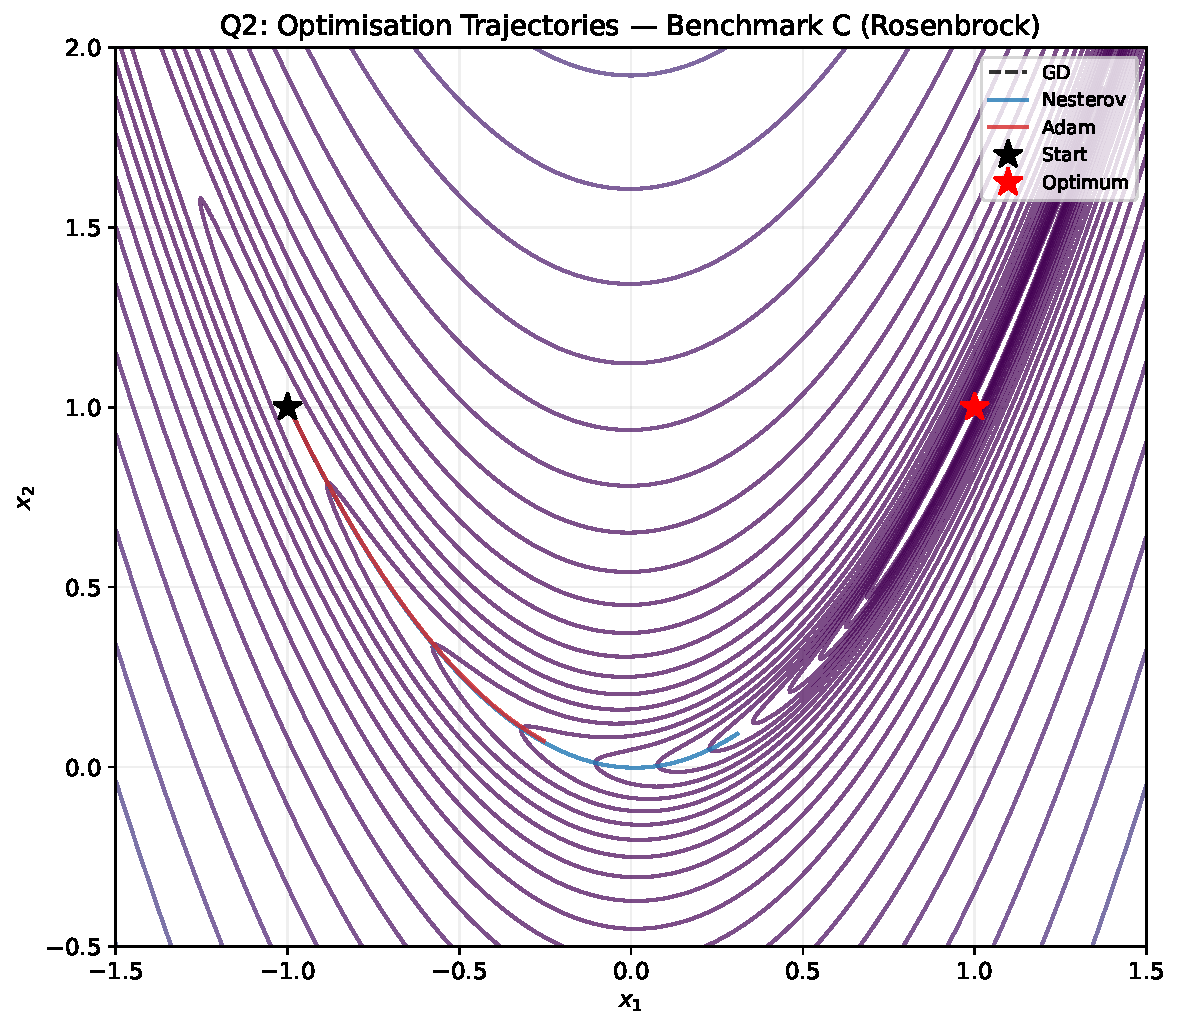
\includegraphics[width=0.88\textwidth]{figures/q2_contour_C.pdf}
\caption{Q2: Trajectories on Benchmark C. All methods descend quickly to the valley floor but differ in their progress \emph{along} the valley. Nesterov's momentum builds acceleration in the consistent valley-floor direction, while GD's constant step size limits valley traversal speed.}
\label{fig:q2_contour_C}
\end{figure}

\subsection{Mini-Batch Stochastic Gradient Descent}

Mini-batch SGD on Benchmark A uses learning rate $\alpha = 0.06$, batch sizes $b \in \{5, 40\}$, 50 epochs, with data shuffled at every epoch.

\begin{algorithm}[H]
\caption{Mini-Batch SGD}
\label{alg:sgd}
\begin{algorithmic}[1]
\Require Data $(X, y)$, initial $\theta_0$, learning rate $\alpha$, batch size $b$, epochs $E$
\For{$e = 1, 2, \ldots, E$}
    \State Randomly permute data indices
    \For{each mini-batch $\mathcal{B}$ of size $b$}
        \State $g \gets \frac{1}{b} X_{\mathcal{B}}^T(X_{\mathcal{B}}\theta - y_{\mathcal{B}})$
        \State $\theta \gets \theta - \alpha\, g$
    \EndFor
\EndFor
\end{algorithmic}
\end{algorithm}

\begin{figure}[H]
\centering
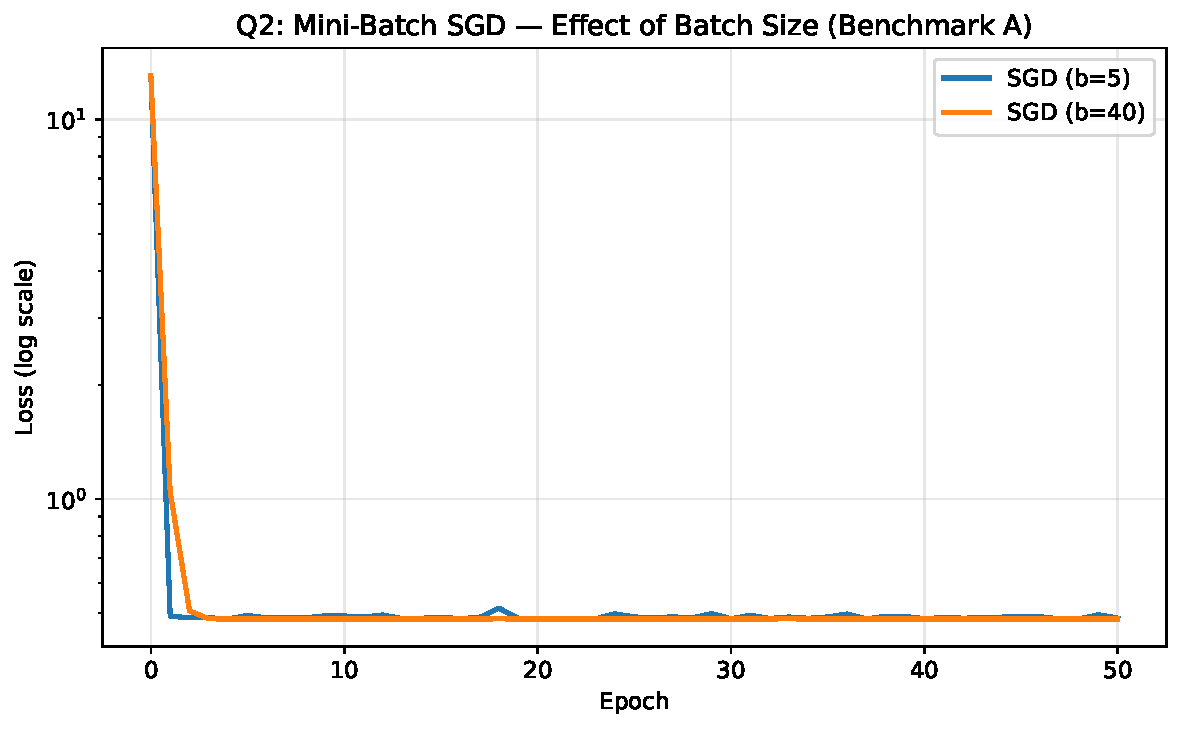
\includegraphics[width=0.85\textwidth]{figures/q2_sgd_batch.pdf}
\caption{Q2: Mini-batch SGD with different batch sizes. With $b = 5$, each epoch performs $1000/5 = 200$ updates, providing faster per-epoch convergence but higher gradient variance. With $b = 40$, each epoch has $1000/40 = 25$ updates, resulting in smoother but slower per-epoch progress. The smaller batch size reaches lower loss faster in terms of epochs due to more frequent updates, but exhibits more oscillation near the minimum because each mini-batch gradient deviates more from the true gradient.}
\label{fig:q2_sgd_batch}
\end{figure}

\subsection{SGD with Increased Noise}

The experiment is repeated with output noise scaled by a factor of 6 ($\sigma = 6$ vs $\sigma = 1$).

\begin{figure}[H]
\centering
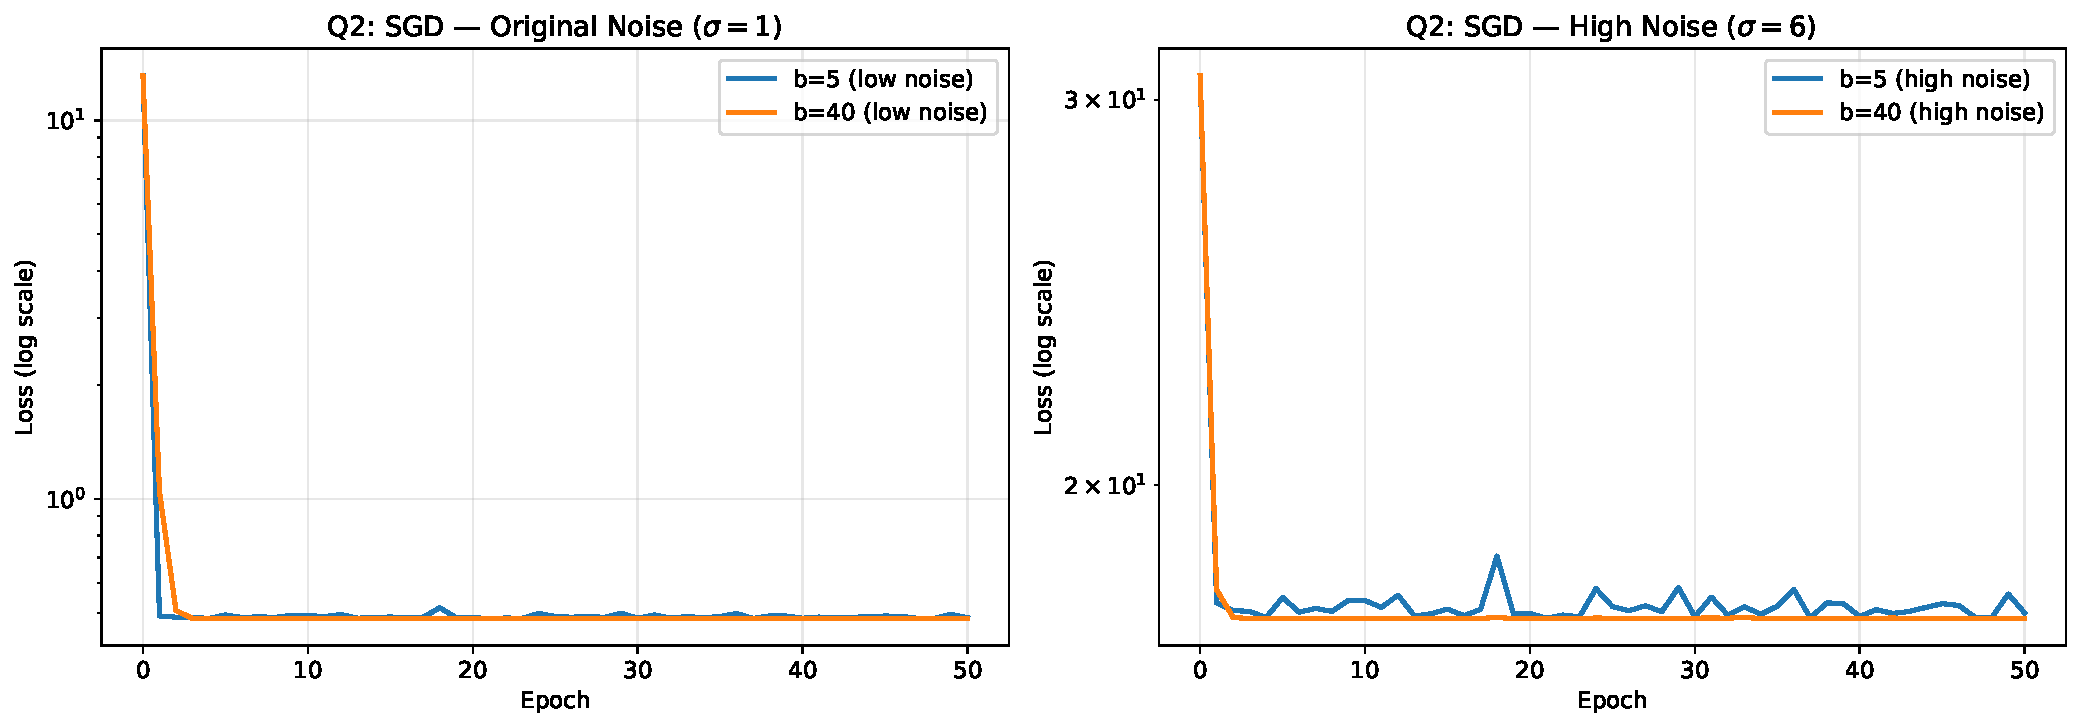
\includegraphics[width=\textwidth]{figures/q2_sgd_noisy.pdf}
\caption{Q2: Effect of noise on SGD convergence. Left: original noise ($\sigma = 1$). Right: high noise ($\sigma = 6$). Increasing the noise by factor 6 raises the irreducible loss floor by factor $\sim 36$ (since $J^{\star} \propto \sigma^2$). Under high noise, both batch sizes converge to approximately the same elevated floor ($J^{\star} \approx 18$), and the relative advantage of smaller batches diminishes --- the gradient noise from the observation model dominates the mini-batch sampling noise.}
\label{fig:q2_sgd_noisy}
\end{figure}

% ============================================================
\section{Question 3: Newton's Method and Local Approximation \hfill [30 marks]}
\label{sec:q3}
% ============================================================

\subsection{Local Approximations of $g(x) = x^4$}

\textbf{First-order (Taylor) approximation} around $x_0 = 0.25$:
\begin{equation}
g(x) \approx g(x_0) + g'(x_0)(x - x_0) = 0.25^4 + 4 \cdot 0.25^3\,(x - 0.25) = 0.0039 + 0.0625(x - 0.25).
\end{equation}

\textbf{Second-order approximation:}
\begin{equation}
g(x) \approx g(x_0) + g'(x_0)(x - x_0) + \tfrac{1}{2}g''(x_0)(x - x_0)^2 = 0.0039 + 0.0625(x - 0.25) + 0.375(x - 0.25)^2.
\end{equation}

The Newton update minimises the second-order approximation, yielding $x_{k+1} = x_k - g'(x_k)/g''(x_k)$. This corresponds to stepping to the stationary point of the local quadratic model.

\begin{figure}[H]
\centering
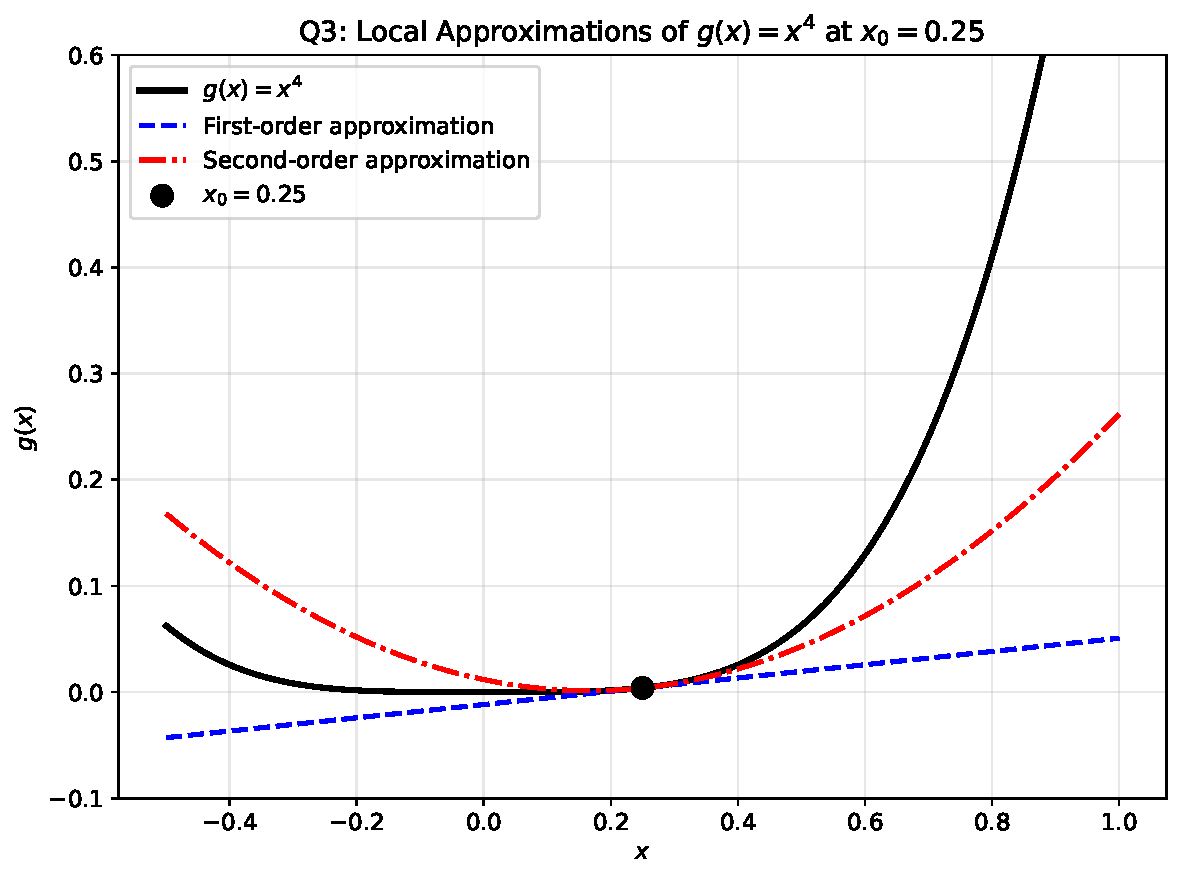
\includegraphics[width=0.85\textwidth]{figures/q3_approximation.pdf}
\caption{Q3: Local approximations of $g(x) = x^4$ at $x_0 = 0.25$. The first-order approximation (tangent line) captures only the local slope and deviates rapidly from the true function. The second-order approximation (parabola) captures the curvature and fits well in a neighbourhood of $x_0$. The minimum of the parabola provides a better estimate of the function's minimum than a gradient step, motivating Newton's method.}
\label{fig:q3_approx}
\end{figure}

\subsection{Newton's Method}

\begin{algorithm}[H]
\caption{Newton's Method with Damping}
\label{alg:newton}
\begin{algorithmic}[1]
\Require Initial point $x_0$, step size $\alpha$, damping $\lambda$, iterations $N$
\For{$k = 0, 1, \ldots, N-1$}
    \State $g_k \gets \nabla f(x_k)$
    \State $H_k \gets \nabla^2 f(x_k) + \lambda I$ \Comment{Regularised Hessian}
    \State $p_k \gets H_k^{-1}\, g_k$ \Comment{Newton direction}
    \State $x_{k+1} \gets x_k - \alpha\, p_k$
\EndFor
\end{algorithmic}
\end{algorithm}

Settings: GD uses 80 iterations; Newton uses 20 iterations with Hessian damping $\lambda = 10^{-8}$.

\begin{table}[H]
\centering
\caption{Q3: Hyperparameters for GD and Newton.}
\label{tab:q3_params}
\begin{tabular}{lcccccc}
\toprule
 & \multicolumn{2}{c}{\textbf{Bench.\ A}} & \multicolumn{2}{c}{\textbf{Bench.\ B}} & \multicolumn{2}{c}{\textbf{Bench.\ C}} \\
\cmidrule(lr){2-3} \cmidrule(lr){4-5} \cmidrule(lr){6-7}
 & GD & Newton & GD & Newton & GD & Newton \\
\midrule
$\alpha$ & 0.08 & 1.0 & 0.06 & 0.85 & 0.001 & 0.22 \\
Iterations & 80 & 20 & 80 & 20 & 80 & 20 \\
\bottomrule
\end{tabular}
\end{table}

\subsection{Convergence Comparison}

\begin{figure}[H]
\centering
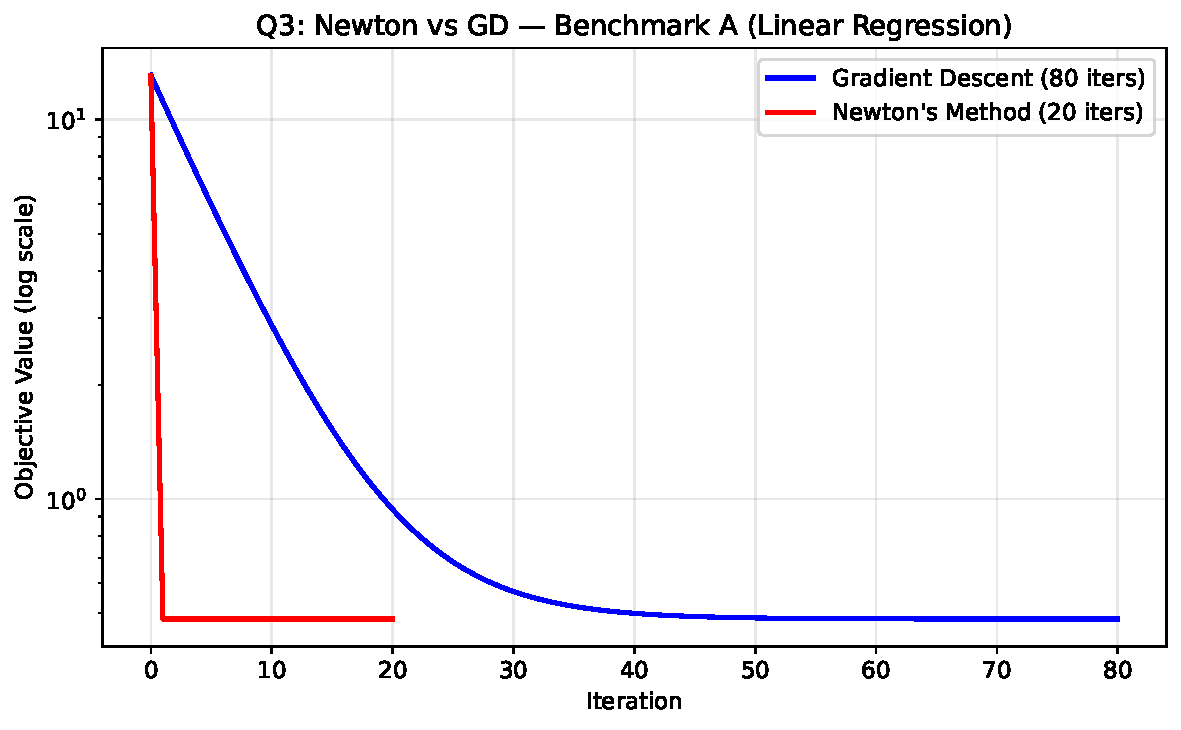
\includegraphics[width=0.85\textwidth]{figures/q3_fval_A.pdf}
\caption{Q3: Newton vs GD on Benchmark A. Newton's method with $\alpha = 1.0$ converges in \textbf{one iteration} to $J = 0.4826$. This is expected: for a quadratic loss $J(\theta) = \frac{1}{2}\theta^T H \theta - b^T\theta + c$, the Newton step $\theta_{k+1} = \theta_k - H^{-1}\nabla J(\theta_k)$ yields the exact minimiser $\theta^{\star} = H^{-1}b$ in a single step. GD requires 80 iterations to reach comparable accuracy.}
\label{fig:q3_fval_A}
\end{figure}

\begin{figure}[H]
\centering
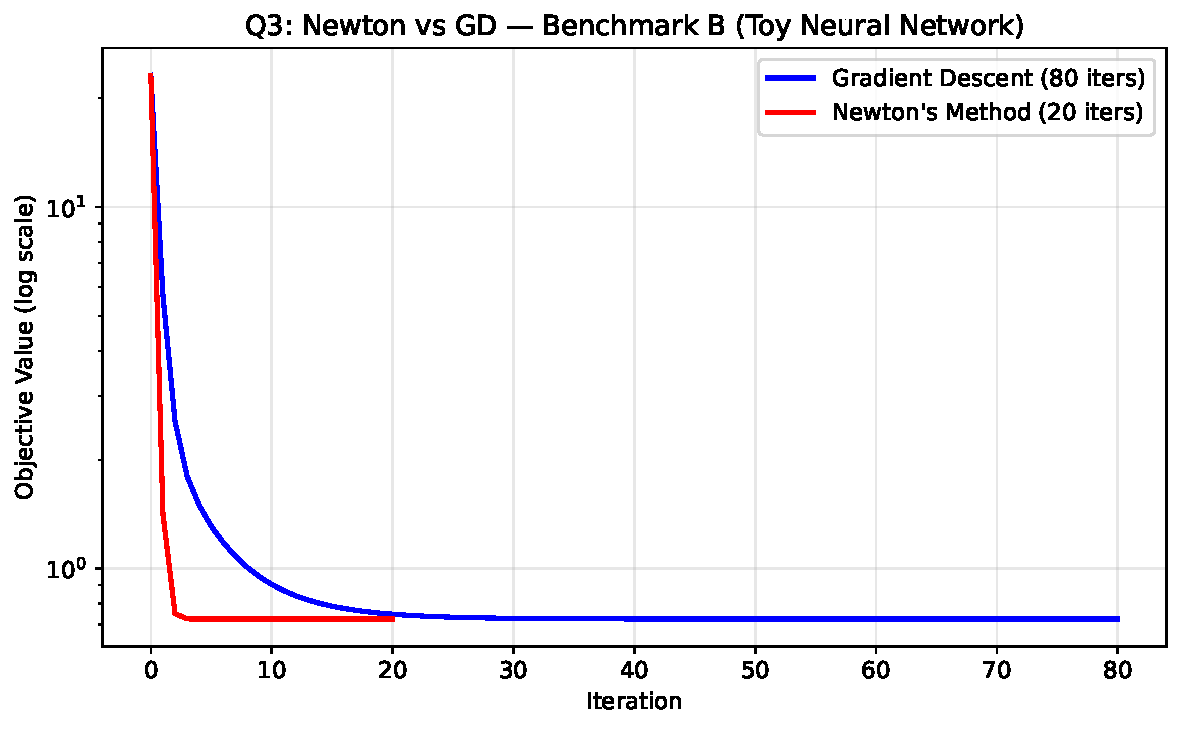
\includegraphics[width=0.85\textwidth]{figures/q3_fval_B.pdf}
\caption{Q3: Newton vs GD on Benchmark B. Newton converges in few iterations due to the near-quadratic structure. The Hessian $H = \text{diag}(2 - \sin(x_1), 10)$ varies slowly, so Newton's curvature information remains accurate across steps. Final value: Newton $f = 0.7244$, matching GD but in far fewer iterations.}
\label{fig:q3_fval_B}
\end{figure}

\begin{figure}[H]
\centering
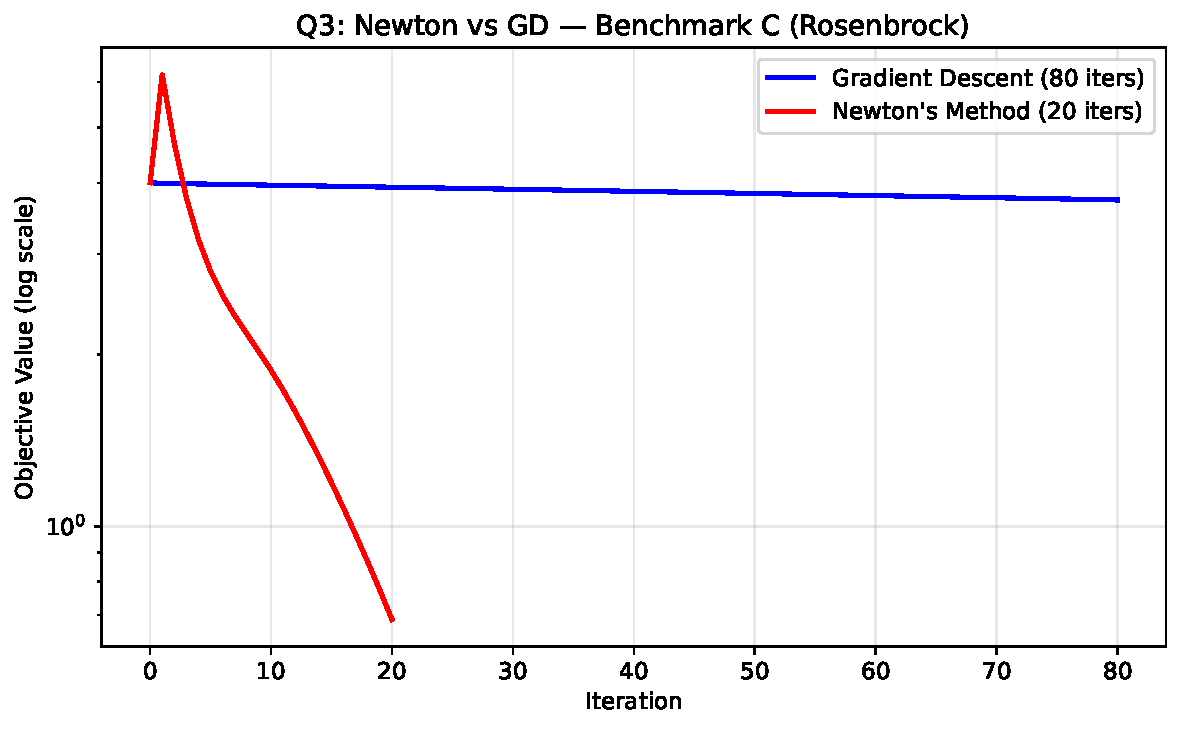
\includegraphics[width=0.85\textwidth]{figures/q3_fval_C.pdf}
\caption{Q3: Newton vs GD on Benchmark C. Newton with $\alpha = 0.22$ reaches $f = 0.686$ in 20 iterations, a dramatic improvement over GD's $f = 3.732$ in 80 iterations. The damped step ($\alpha = 0.22 < 1$) is necessary because the Rosenbrock Hessian changes rapidly, and full Newton steps would overshoot. The Hessian's curvature information allows Newton to step along the valley efficiently rather than bouncing off the walls.}
\label{fig:q3_fval_C}
\end{figure}

\begin{table}[H]
\centering
\caption{Q3: Final objective values and converged positions.}
\label{tab:q3_final}
\begin{tabular}{lcccc}
\toprule
\textbf{Benchmark} & \textbf{GD $f$ (80 it.)} & \textbf{Newton $f$ (20 it.)} & \textbf{Newton final $x$} \\
\midrule
A & 0.4827 & 0.4826 & $(3.028, 4.017)$ \\
B & 0.7244 & 0.7244 & $(0.582, 2.000)$ \\
C & 3.7319 & 0.6864 & $(0.183, 0.020)$ \\
\bottomrule
\end{tabular}
\end{table}

\subsection{Contour Trajectories}

\begin{figure}[H]
\centering
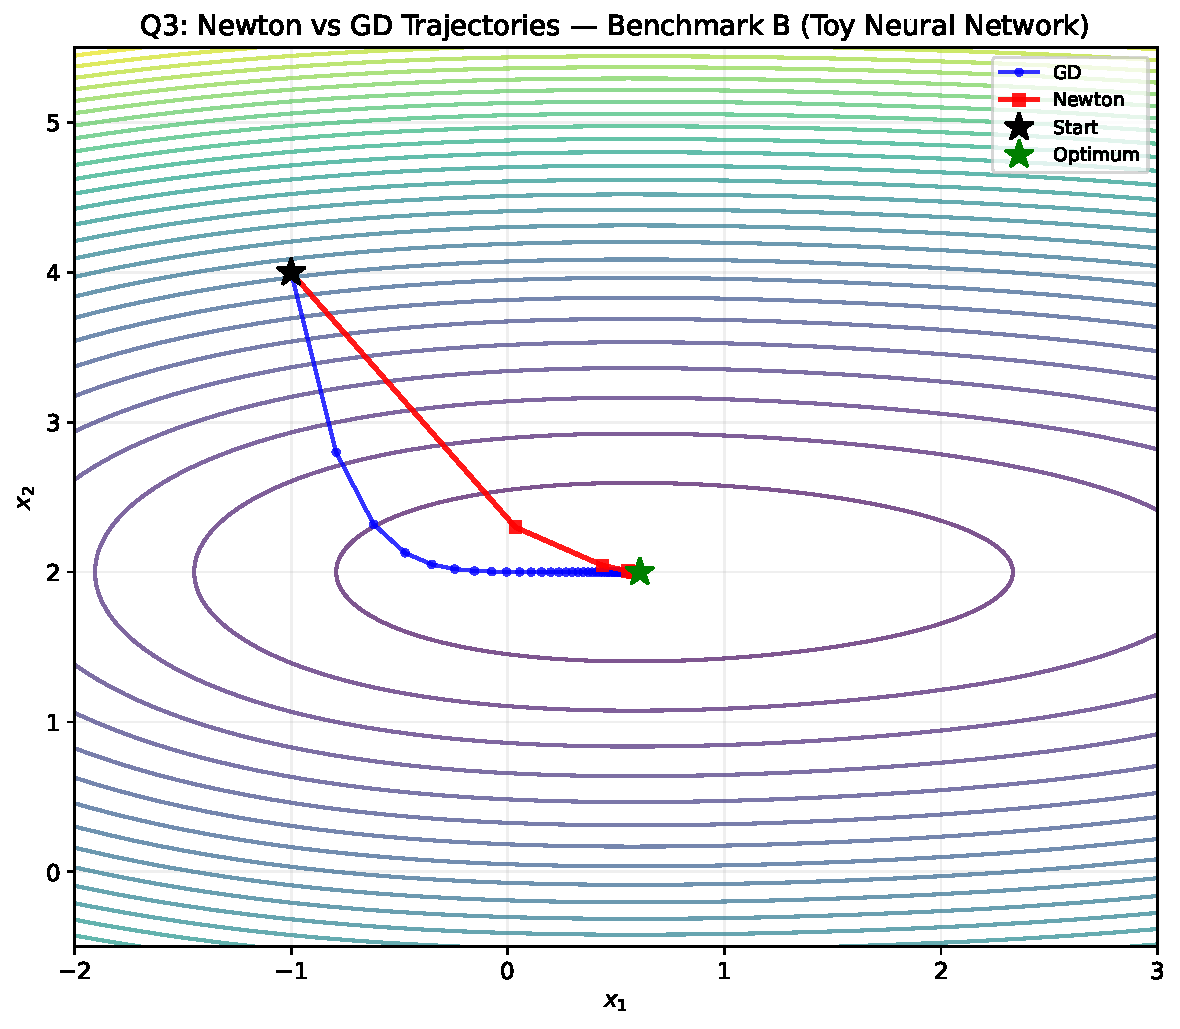
\includegraphics[width=0.88\textwidth]{figures/q3_contour_B.pdf}
\caption{Q3: Newton vs GD trajectories on Benchmark B. Newton takes large, well-directed steps that account for the curvature difference between coordinates, reaching the minimum in $\sim$5 steps. GD takes many small steps, with its trajectory reflecting the anisotropic curvature --- the $x_2$ component converges first (steeper curvature), then $x_1$ follows.}
\label{fig:q3_contour_B}
\end{figure}

\begin{figure}[H]
\centering
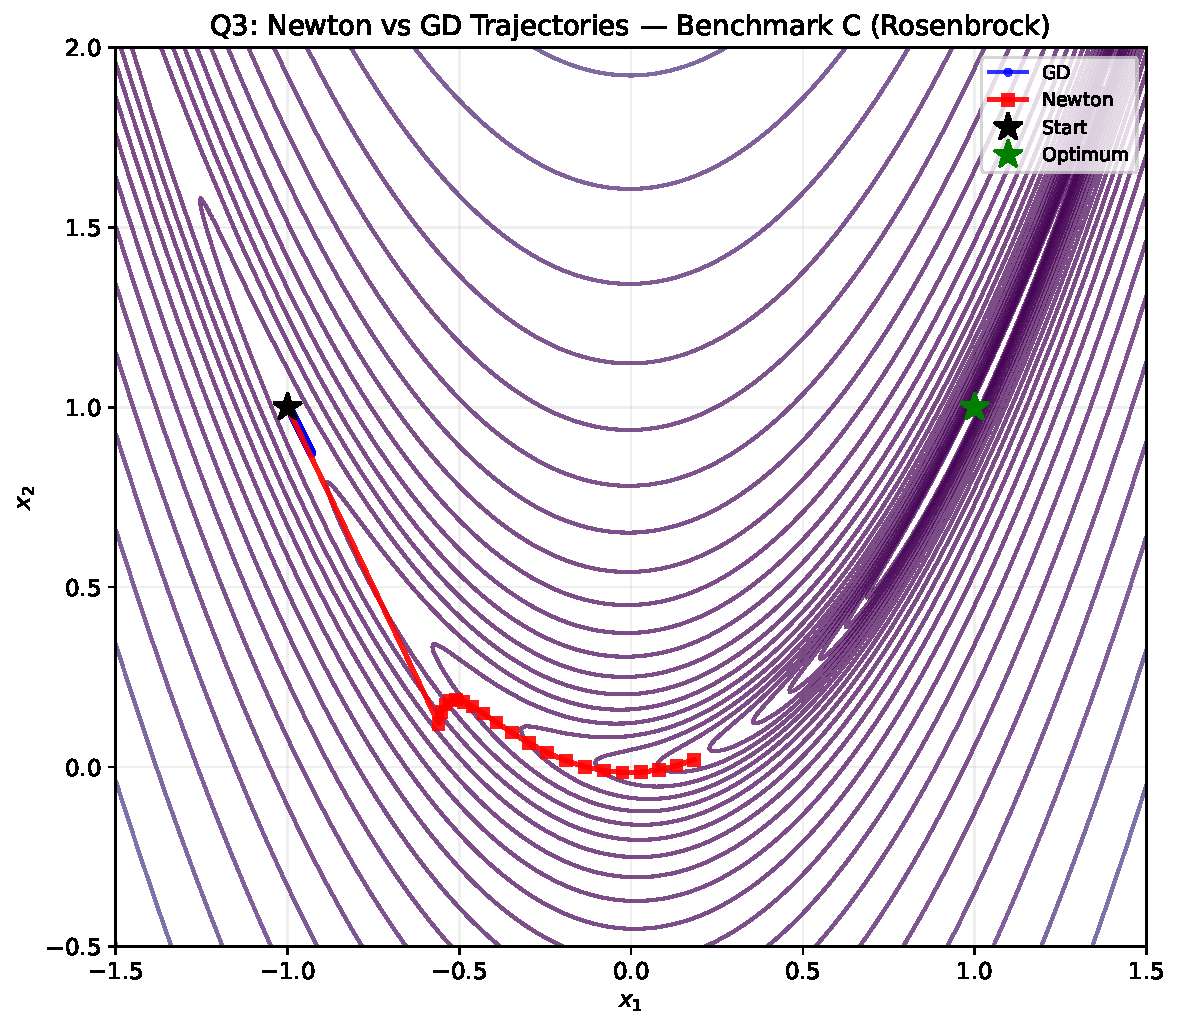
\includegraphics[width=0.88\textwidth]{figures/q3_contour_C.pdf}
\caption{Q3: Newton vs GD trajectories on Rosenbrock. Newton's trajectory follows the valley floor more closely by using local curvature information from the Hessian. GD is constrained to tiny steps ($\alpha = 0.001$) to maintain stability, barely advancing in 80 iterations.}
\label{fig:q3_contour_C}
\end{figure}

\subsection{Update Magnitude}

\begin{figure}[H]
\centering
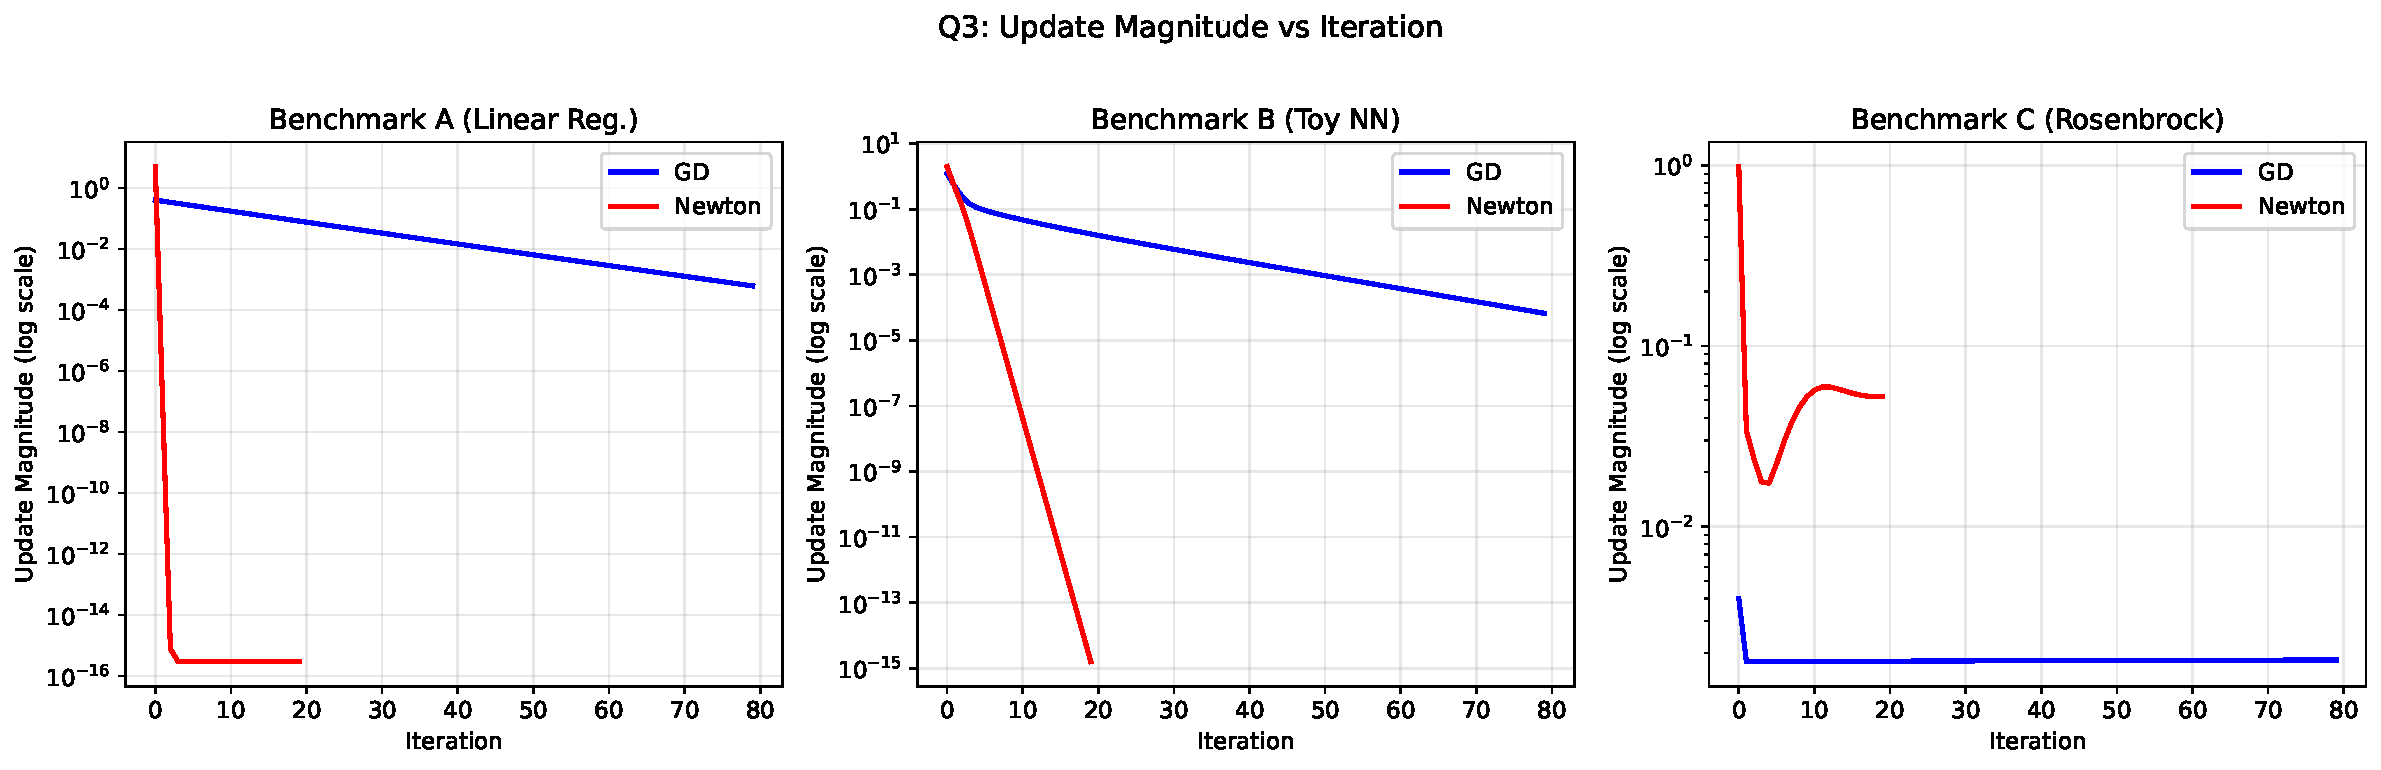
\includegraphics[width=\textwidth]{figures/q3_update_magnitude.pdf}
\caption{Q3: Update magnitude $\|x_{k+1} - x_k\|$ vs iteration for GD and Newton across all three benchmarks. Newton's update magnitude decreases rapidly --- characteristic of quadratic convergence where $\|x_{k+1} - x^{\star}\| \leq C\|x_k - x^{\star}\|^2$. For Benchmark A, Newton's update drops to machine precision after one step. GD's magnitude decreases linearly, reflecting its linear convergence rate. On Rosenbrock, Newton maintains larger updates than GD, indicating more aggressive (and productive) steps.}
\label{fig:q3_update}
\end{figure}

% ============================================================
\section{Question 4: Derivative Approximation and Derivative-Free Optimisation \hfill [30 marks]}
\label{sec:q4}
% ============================================================

\subsection{Part A: Finite Difference and Nesterov Random Search (Benchmark B)}

\subsubsection{Finite Difference Gradient Approximation}

The forward finite-difference approximation replaces each partial derivative with:
\begin{equation}
\frac{\partial f}{\partial x_i}(x) \approx \frac{f(x + \delta e_i) - f(x)}{\delta}.
\end{equation}
The approximation error is $O(\delta)$ (truncation) plus $O(\varepsilon_{\text{machine}}/\delta)$ (numerical precision), yielding an optimal $\delta \sim \sqrt{\varepsilon_{\text{machine}}} \approx 10^{-8}$. The assignment tests $\delta = 0.05$ (good) and $\delta = 0.8$ (poor).

\subsubsection{Nesterov Random Search}

\begin{algorithm}[H]
\caption{Nesterov Random Search}
\label{alg:nrs}
\begin{algorithmic}[1]
\Require Initial point $x_0$, step size $\alpha$, perturbation $\delta$, iterations $N$
\For{$k = 0, 1, \ldots, N-1$}
    \State Sample $u_k \sim \mathcal{N}(0, I)$, normalise: $u_k \gets u_k / \|u_k\|$
    \State $\hat{g}_k \gets \dfrac{f(x_k + \delta u_k) - f(x_k)}{\delta}\, u_k$
    \State $x_{k+1} \gets x_k - \alpha\, \hat{g}_k$
\EndFor
\end{algorithmic}
\end{algorithm}

This zeroth-order method estimates a directional derivative along a random direction, requiring only \emph{two} function evaluations per iteration regardless of dimension, making it dimension-independent in cost per step.

\subsubsection{Results}

\begin{figure}[H]
\centering
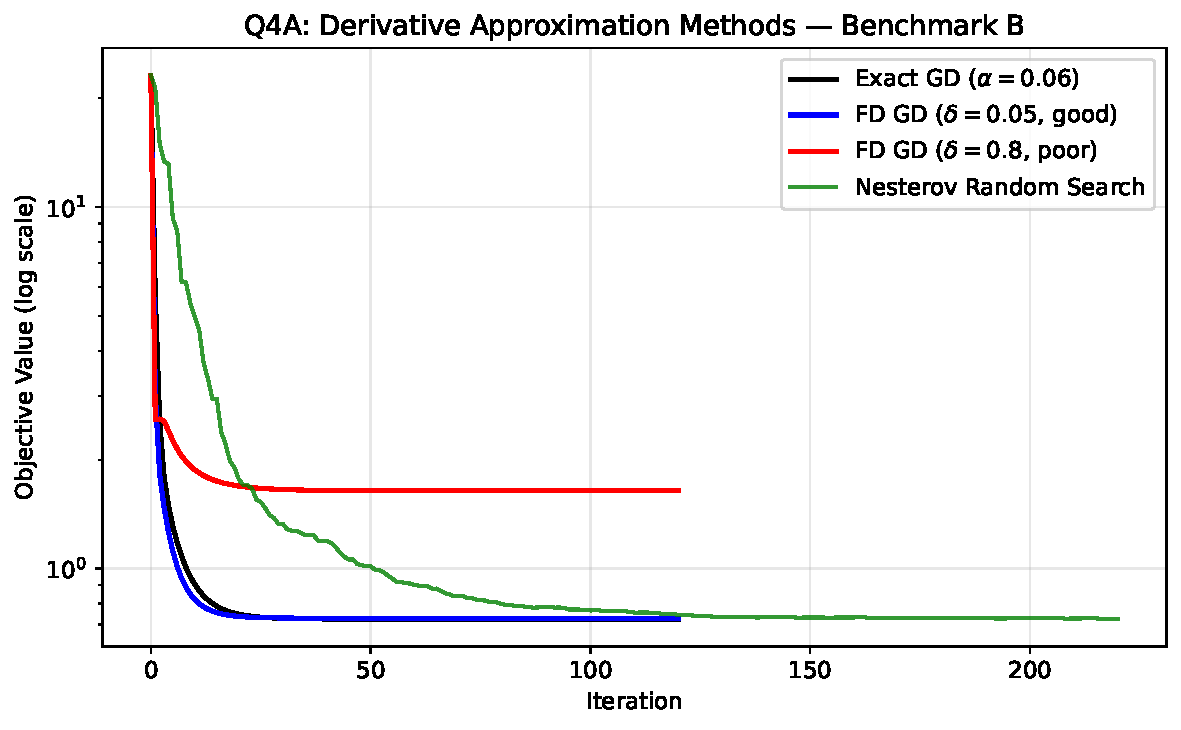
\includegraphics[width=0.85\textwidth]{figures/q4_fval_B.pdf}
\caption{Q4A: Convergence comparison on Benchmark B. Exact GD converges fastest. FD GD with $\delta = 0.05$ closely tracks exact GD, confirming the gradient approximation quality. FD GD with $\delta = 0.8$ converges poorly due to large truncation error --- the finite-difference step spans a region where the curvature changes significantly. Nesterov random search converges slowest: using a single random direction per step provides only a noisy one-dimensional projection of the gradient.}
\label{fig:q4_fval_B}
\end{figure}

\begin{figure}[H]
\centering
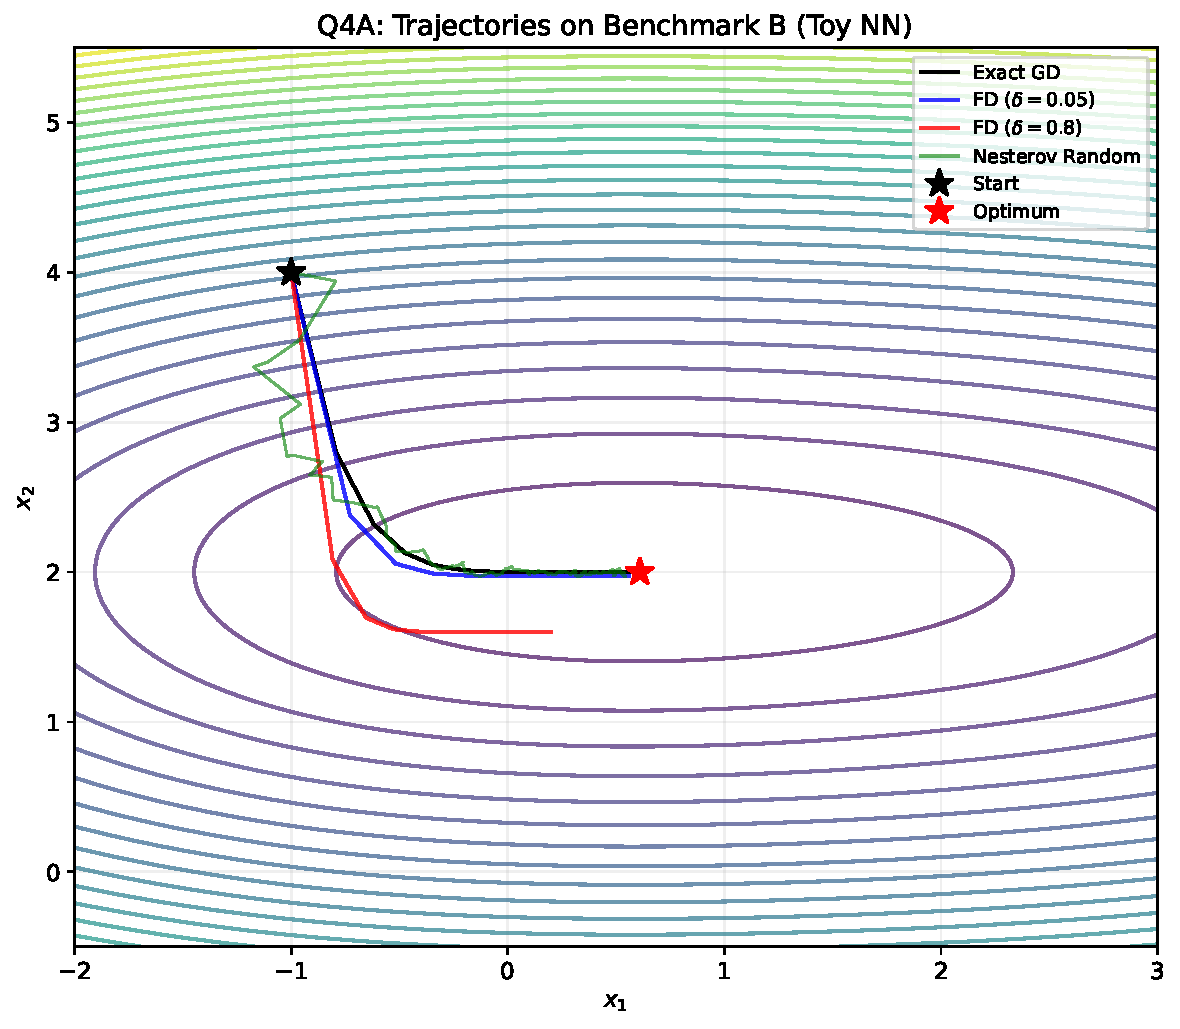
\includegraphics[width=0.88\textwidth]{figures/q4_contour_B.pdf}
\caption{Q4A: Trajectories on Benchmark B. Exact GD and good FD ($\delta = 0.05$) follow nearly identical paths, confirming gradient fidelity. Poor FD ($\delta = 0.8$) deviates due to inaccurate gradient direction. Nesterov random search follows a noisy, wandering path due to random directional sampling.}
\label{fig:q4_contour_B}
\end{figure}

\subsection{Part B: Derivative-Free Methods (Benchmark C)}

\subsubsection{Nelder--Mead Simplex Method}

The Nelder--Mead algorithm maintains a simplex of $n+1 = 3$ vertices in $\mathbb{R}^2$ and iteratively transforms it through four operations: \textbf{reflection} (move worst vertex through the centroid), \textbf{expansion} (if reflection improved, try further), \textbf{contraction} (if reflection worsened, contract towards centroid), and \textbf{shrink} (contract all vertices towards best). No gradient information is required.

Settings: initial simplex step $= 0.35$, iterations $= 160$.

\begin{figure}[H]
\centering
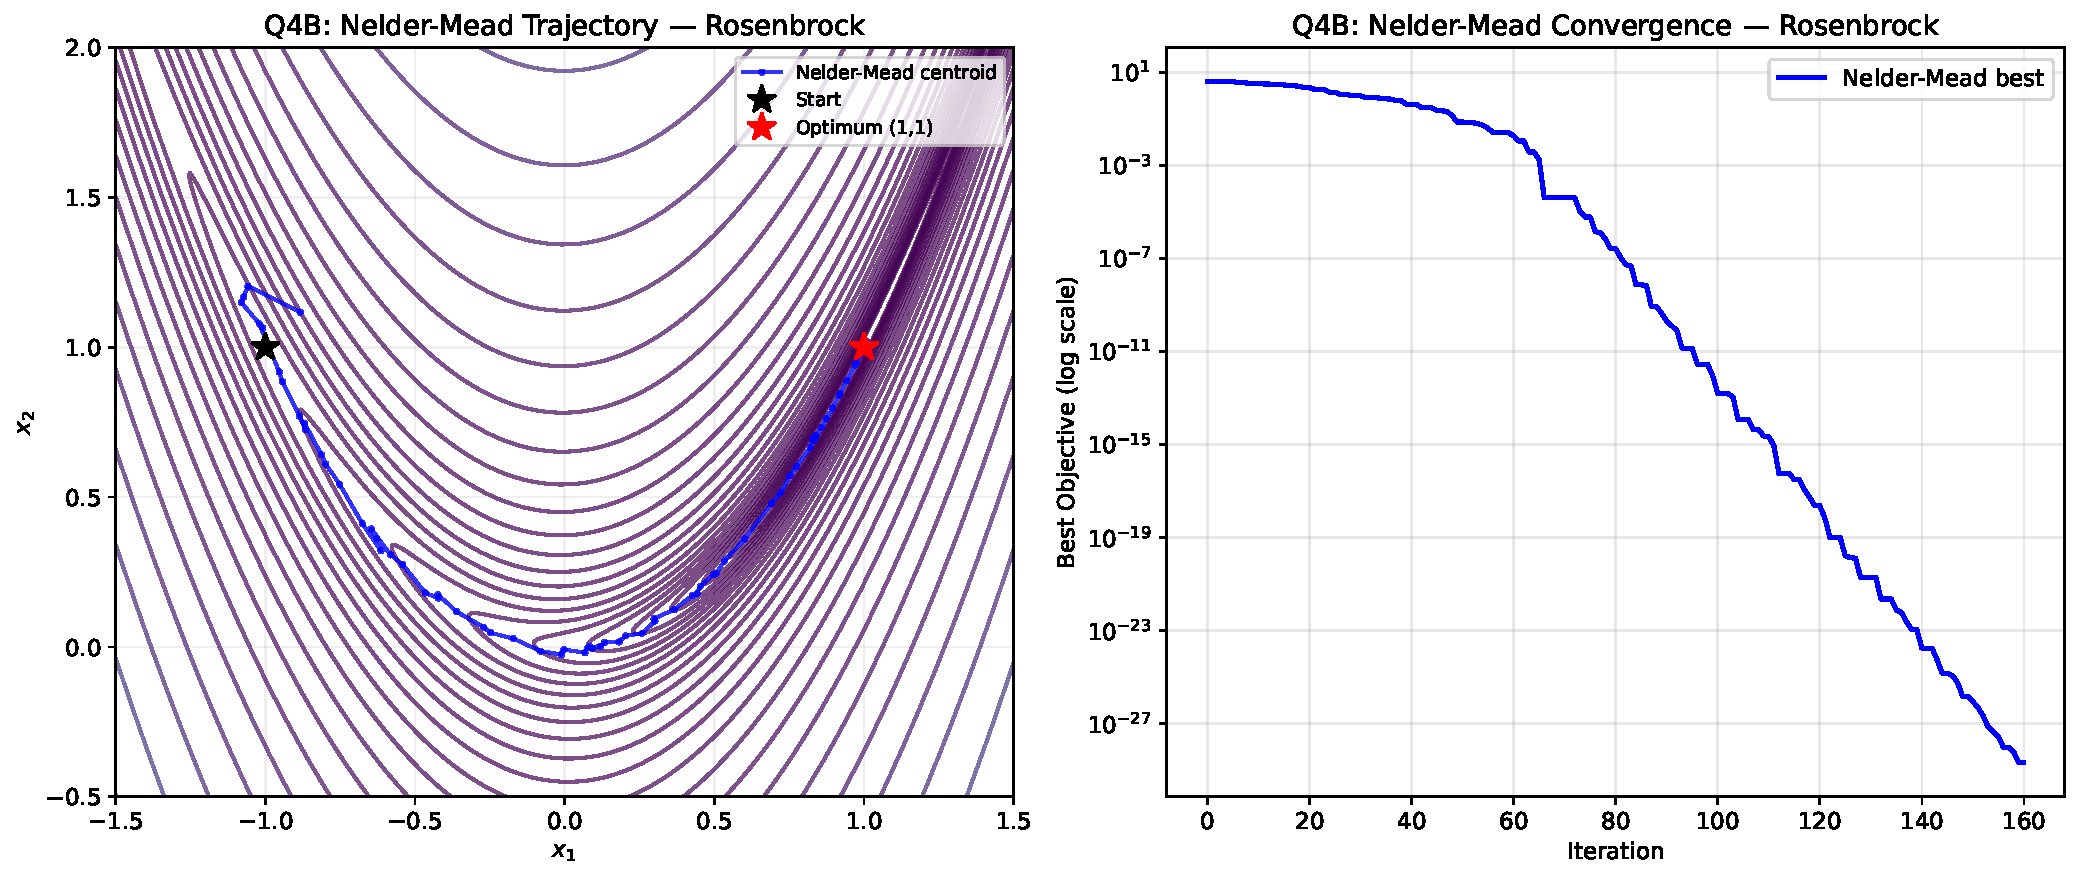
\includegraphics[width=\textwidth]{figures/q4_nelder_mead_C.pdf}
\caption{Q4B: Nelder--Mead on Rosenbrock. Left: the simplex centroid trajectory navigates the curved valley without gradient information, demonstrating that the simplex geometry adapts to the local landscape. Right: the best objective value decreases steadily as the simplex contracts towards the minimum.}
\label{fig:q4_nm}
\end{figure}

\subsubsection{Grid Search}

Grid search evaluates the objective on a uniform $55 \times 55 = 3025$ grid over $x_1 \in [-2, 2]$, $x_2 \in [-1, 3]$.

\begin{figure}[H]
\centering
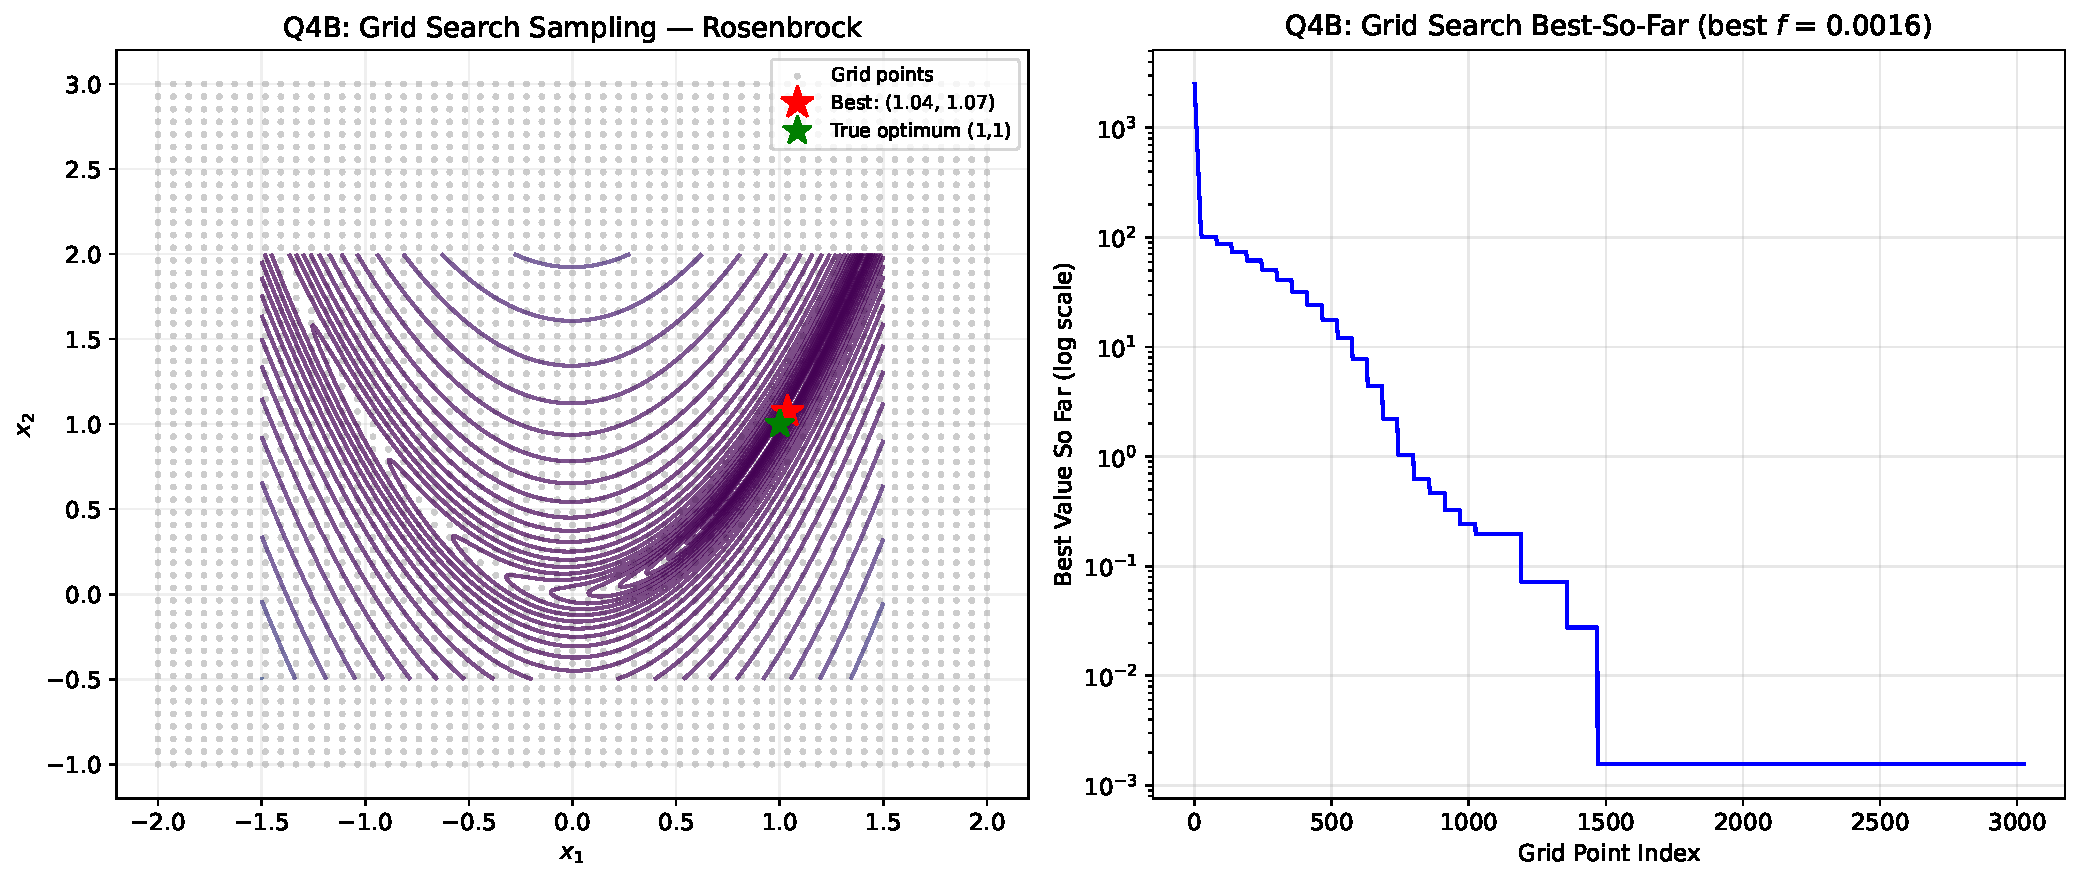
\includegraphics[width=\textwidth]{figures/q4_grid_search_C.pdf}
\caption{Q4B: Grid search on Rosenbrock. Left: the 3025 grid points cover the search region uniformly. The best point found is near the true optimum. Right: the best-so-far curve shows step-wise improvement as better points are discovered during the scan. Grid search guarantees finding the global optimum to within the grid resolution $\Delta x \approx 0.073$, but requires $O(N^d)$ evaluations, making it impractical for $d > 3$.}
\label{fig:q4_grid}
\end{figure}

\subsection{Computational Comparison}

\begin{table}[H]
\centering
\caption{Q4: Comparison of methods. FE = function evaluations per iteration, $d$ = dimension.}
\label{tab:q4_comparison}
\begin{tabular}{lcccc}
\toprule
\textbf{Method} & \textbf{Gradient Info} & \textbf{FE/iter} & \textbf{Scalability} & \textbf{Accuracy} \\
\midrule
Exact GD & Full gradient & $1 + d$ & Good & High \\
FD GD ($\delta$ small) & Approx.\ gradient & $d + 1$ & Moderate & High \\
FD GD ($\delta$ large) & Poor approx. & $d + 1$ & Moderate & Low \\
Nesterov random & None & 2 & \textbf{Best} & Low \\
Nelder--Mead & None & $\leq 3$ & Low-dim & Moderate \\
Grid search & None & $N^d$ total & Very poor & Grid-limited \\
\bottomrule
\end{tabular}
\end{table}

% ============================================================
\section{Question 5: Constrained Optimisation \hfill [30 marks]}
\label{sec:q5}
% ============================================================

\subsection{Problem Setup}

Minimise Benchmark B subject to $x_1 \geq 0.5$, starting from the infeasible point $x_0 = (0.2, 4.0)$.

\begin{algorithm}[H]
\caption{Projected Gradient Descent}
\label{alg:pgd}
\begin{algorithmic}[1]
\Require Initial point $x_0$, step size $\alpha$, projection $\Pi_{\mathcal{X}}$, iterations $N$
\For{$k = 0, 1, \ldots, N-1$}
    \State $z_{k+1} \gets x_k - \alpha\, \nabla f(x_k)$ \Comment{Unconstrained gradient step}
    \State $x_{k+1} \gets \Pi_{\mathcal{X}}(z_{k+1})$ \Comment{Project: $x_1 \leftarrow \max(0.5,\, x_1)$}
\EndFor
\end{algorithmic}
\end{algorithm}

\begin{algorithm}[H]
\caption{Penalty Method}
\label{alg:penalty}
\begin{algorithmic}[1]
\Require Initial point $x_0$, step size $\alpha$, penalty weight $\lambda$, iterations $N$
\For{$k = 0, 1, \ldots, N-1$}
    \State $F_{\lambda}(x) \gets f(x) + \lambda \max(0,\, -x_1 + 0.5)$ \Comment{Penalised objective}
    \State $x_{k+1} \gets x_k - \alpha\, \nabla F_{\lambda}(x_k)$
\EndFor
\end{algorithmic}
\end{algorithm}

Settings: Projected GD ($\alpha = 0.08$), Penalty with $\lambda \in \{0.15, 1.8, 4.5\}$ ($\alpha = 0.05$ for $\lambda \leq 1.8$; $\alpha = 0.03$ for $\lambda = 4.5$), unconstrained GD ($\alpha = 0.07$). All run for 100 iterations.

\subsection{Results}

\begin{figure}[H]
\centering
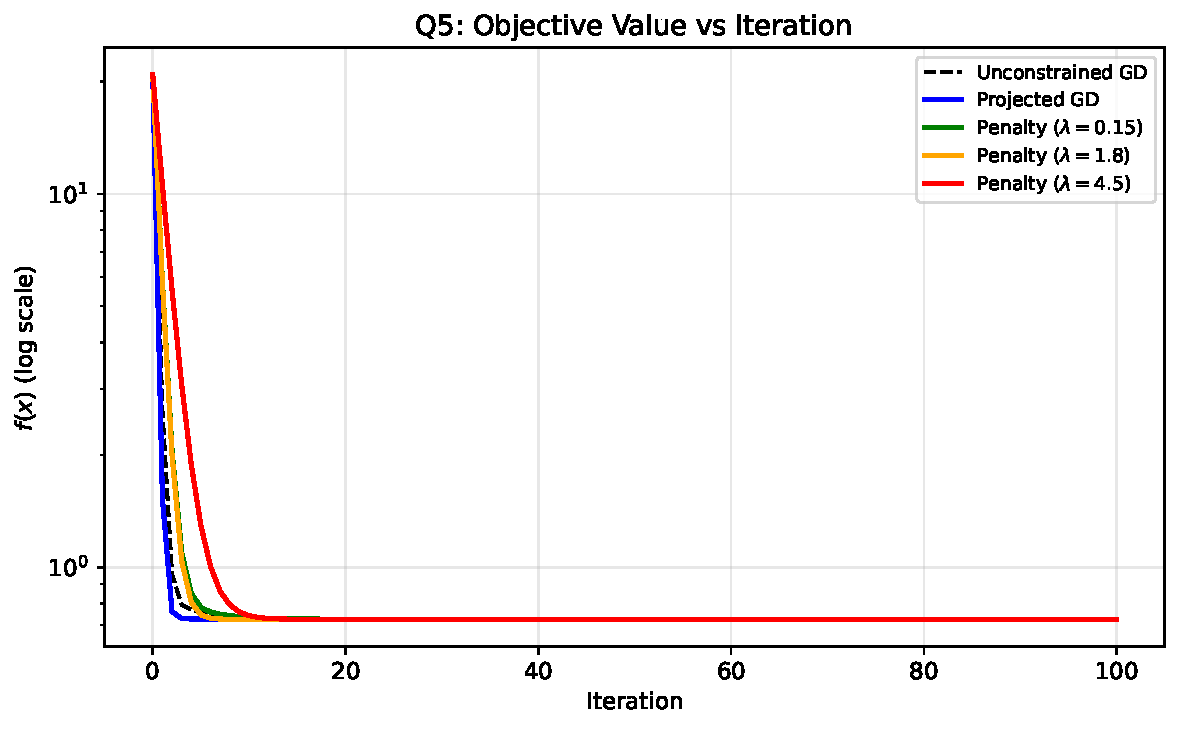
\includegraphics[width=0.85\textwidth]{figures/q5_fval.pdf}
\caption{Q5: Objective value vs iteration. Projected GD converges to the constrained minimum $f \approx 0.7244$ at $(0.582, 2.0)$. The penalty methods with larger $\lambda$ produce trajectories that approach the same constrained minimum, while $\lambda = 0.15$ settles at a point with residual constraint violation.}
\label{fig:q5_fval}
\end{figure}

\begin{figure}[H]
\centering
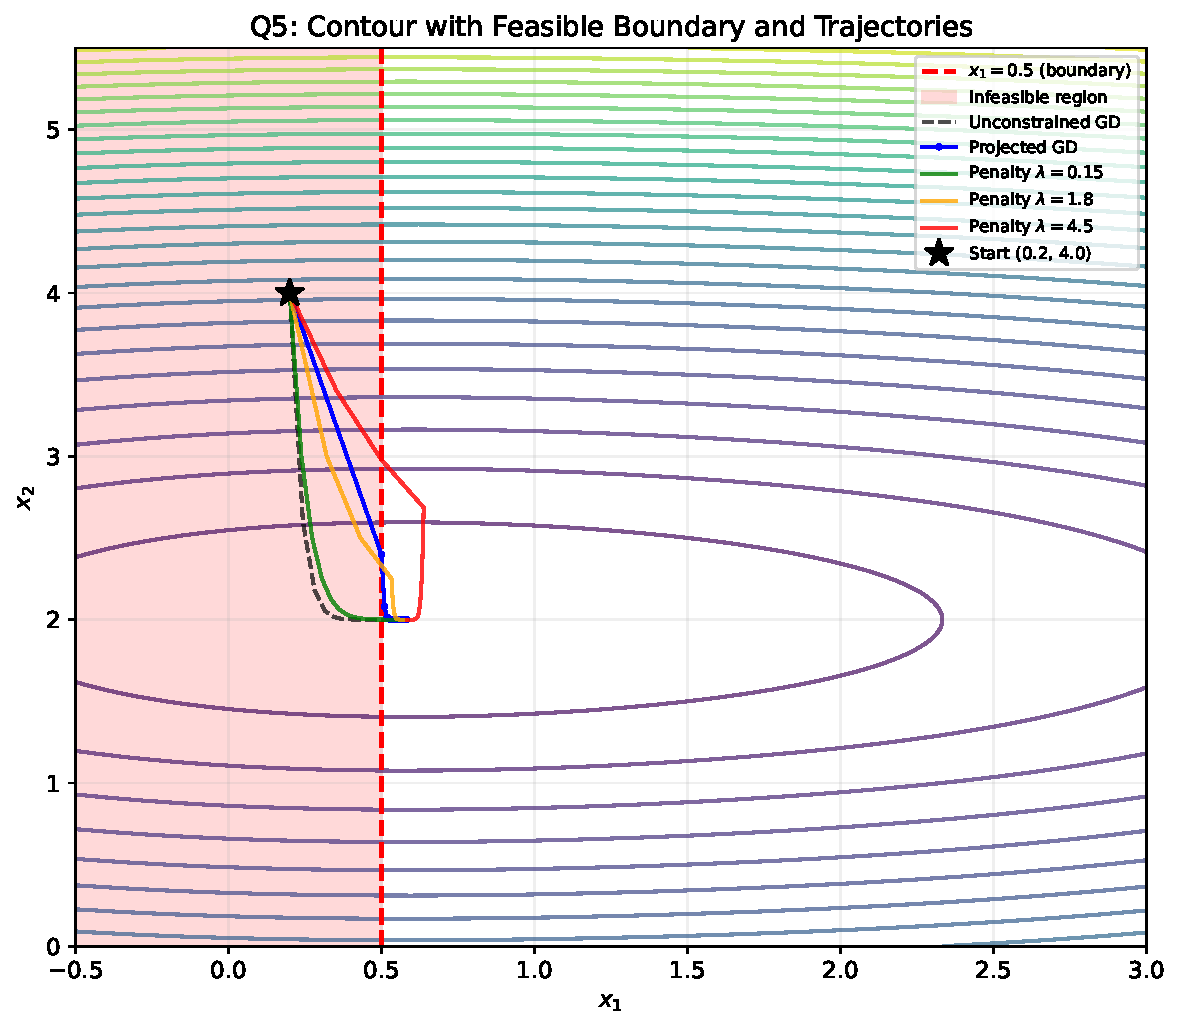
\includegraphics[width=0.88\textwidth]{figures/q5_contour.pdf}
\caption{Q5: Contour plot with constraint boundary $x_1 = 0.5$ (dashed red line) and infeasible region (shaded). The starting point $(0.2, 4.0)$ is infeasible. Projected GD immediately clips to $x_1 = 0.5$ and then optimises within the feasible set. The unconstrained GD path crosses into the infeasible region. Penalty methods with increasing $\lambda$ are progressively steered towards feasibility.}
\label{fig:q5_contour}
\end{figure}

\subsection{Constraint Violation Analysis}

\begin{figure}[H]
\centering
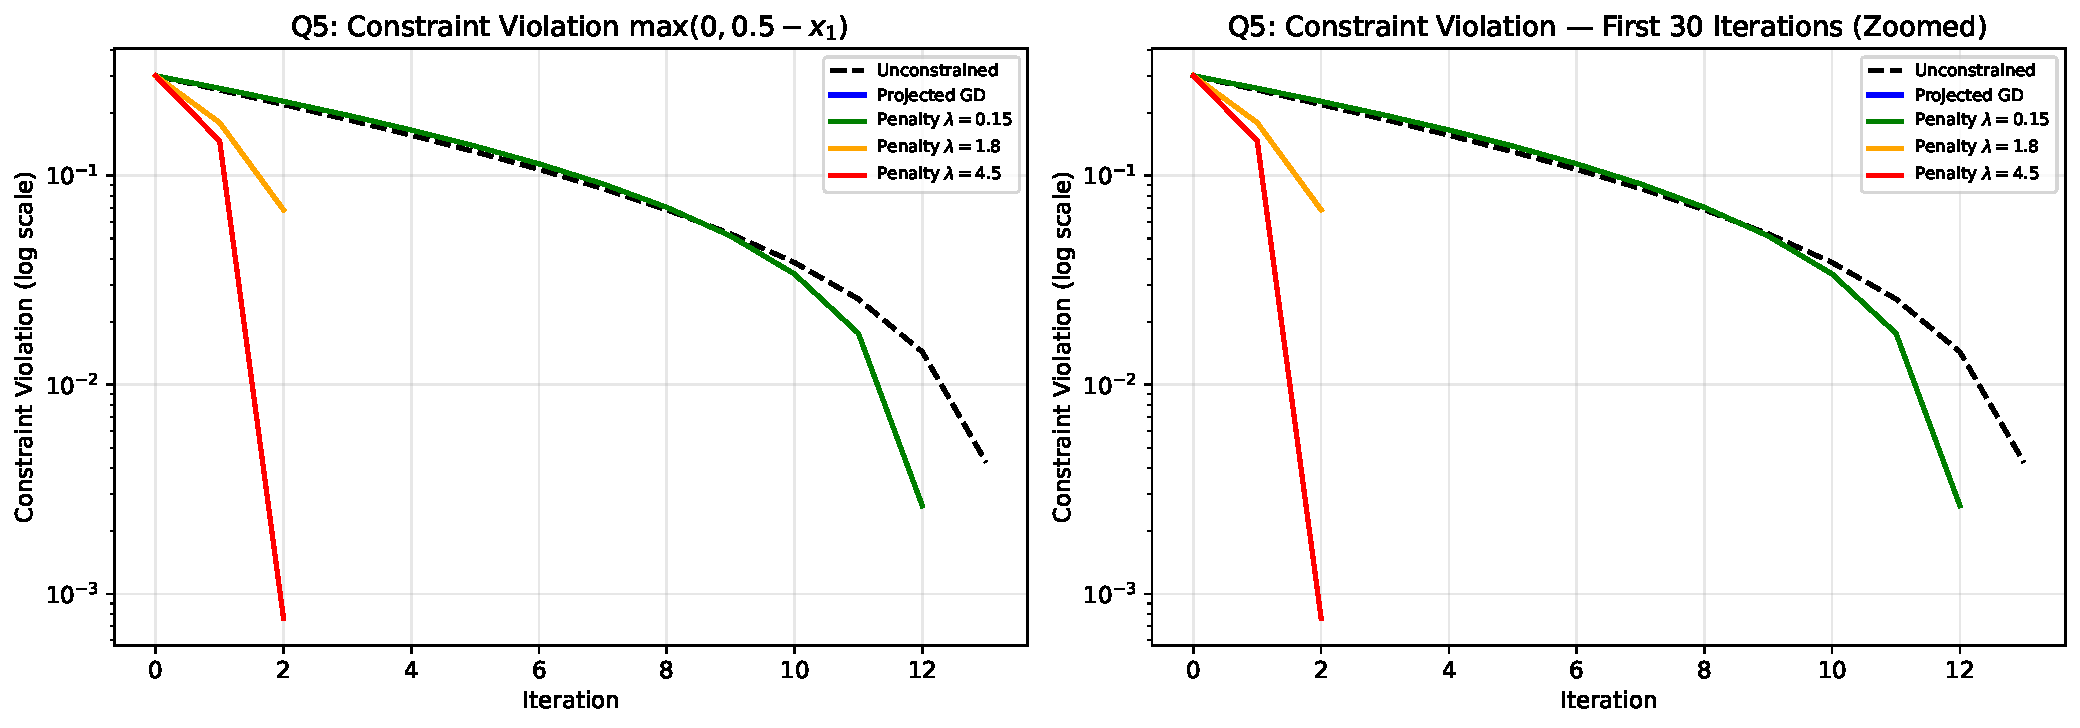
\includegraphics[width=\textwidth]{figures/q5_violation.pdf}
\caption{Q5: Constraint violation $\max(0, 0.5 - x_1)$ on logarithmic scale. Left: full 100 iterations. Right: first 30 iterations (zoomed). Projected GD achieves \textbf{zero violation from iteration 1} --- the projection operator enforces $x_1 \geq 0.5$ as a hard constraint at every step. Penalty method with $\lambda = 4.5$ achieves feasibility within $\sim$10 iterations. With $\lambda = 0.15$, the penalty gradient is too weak relative to the objective gradient, and feasibility is enforced slowly or incompletely.}
\label{fig:q5_violation}
\end{figure}

\subsection{Comparative Discussion}

\begin{table}[H]
\centering
\caption{Q5: Final positions and constraint violations after 100 iterations.}
\label{tab:q5_final}
\begin{tabular}{lccc}
\toprule
\textbf{Method} & \textbf{Final $x$} & \textbf{$f(x)$} & \textbf{Violation} \\
\midrule
Projected GD & $(0.582, 2.000)$ & 0.7244 & 0.0000 \\
Penalty $\lambda = 4.5$ & $(0.583, 2.000)$ & 0.7244 & 0.0000 \\
\bottomrule
\end{tabular}
\end{table}

\textbf{Projected GD} enforces feasibility immediately at every iteration. This is the fundamental advantage: feasibility is a hard constraint, not negotiable. The cost is requiring a projection oracle, which for simple constraints like $x_1 \geq 0.5$ is trivial ($\max$ operation) but can be expensive for complex constraint sets.

\textbf{Penalty methods} trade exact feasibility for simplicity: only a modified gradient is needed. The weight $\lambda$ controls the trade-off. Small $\lambda$ under-penalises violations; large $\lambda$ enforces feasibility but requires smaller step sizes to maintain stability (here, $\alpha = 0.03$ for $\lambda = 4.5$ vs $\alpha = 0.05$ for $\lambda \leq 1.8$).

% ============================================================
\section{Question 6: Linear Programmes and Frank--Wolfe Algorithm \hfill [30 marks]}
\label{sec:q6}
% ============================================================

\subsection{Feasible Set and Linear Programme}

Feasible set: $\mathcal{X} = \{x \in \mathbb{R}^2 : 0.5 \leq x_1 \leq 5,\ -5 \leq x_2 \leq 10\}$.

\textbf{Linear Programme:} For $f(x) = a^T x$ with $a = [1, 2]^T$, the minimum over $\mathcal{X}$ is obtained by minimising each coordinate independently. Since both components of $a$ are positive, the optimum is at the lower bounds:
\begin{equation}
x^{\star} = (0.5,\, -5), \qquad f^{\star} = 0.5 + 2(-5) = -9.5.
\end{equation}
This illustrates the fundamental theorem of linear programming: the optimum of a linear objective over a bounded polytope is attained at a vertex.

\begin{figure}[H]
\centering
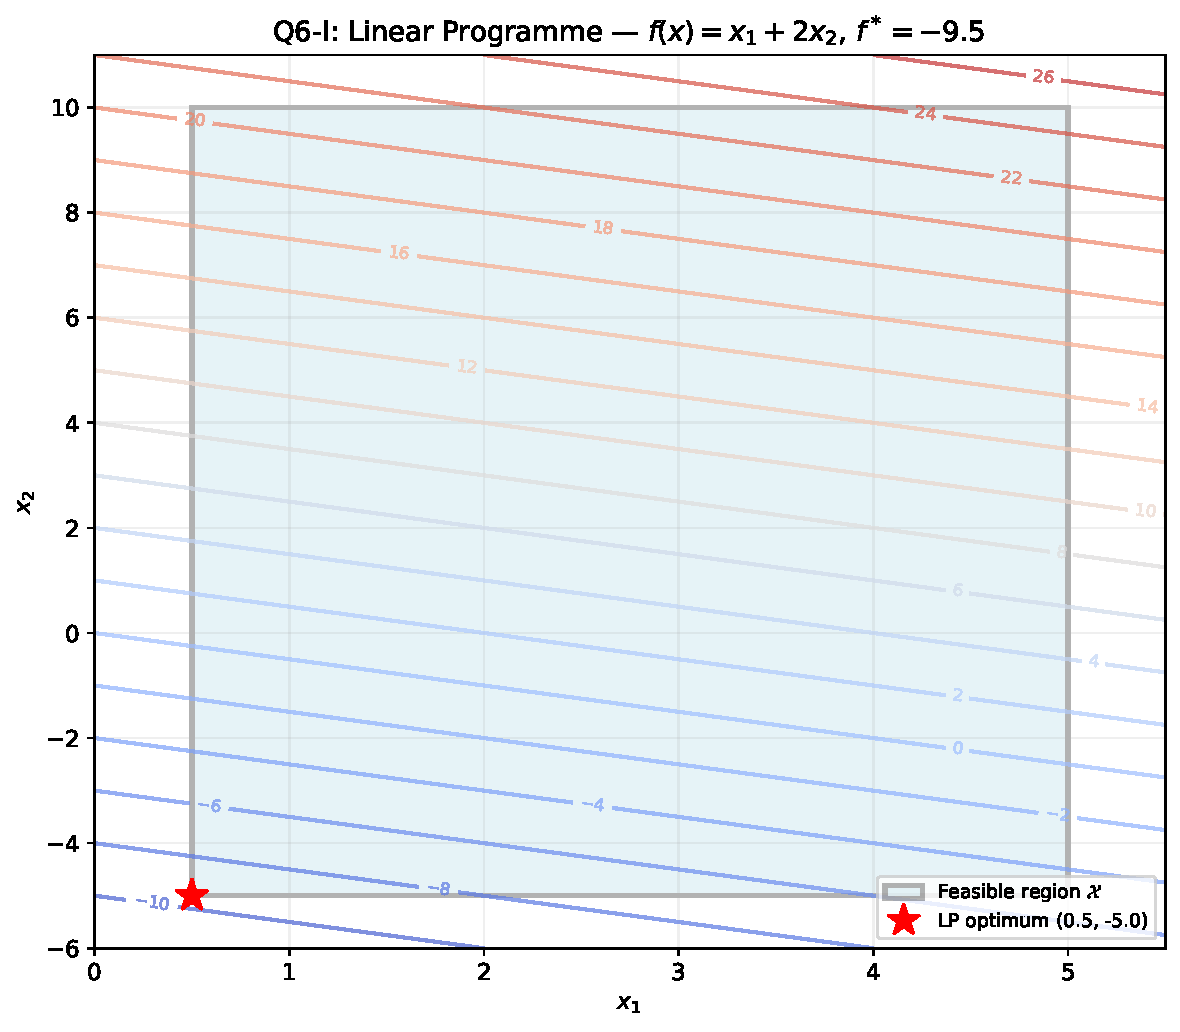
\includegraphics[width=0.85\textwidth]{figures/q6_lp.pdf}
\caption{Q6-I: Feasible region (blue box) and linear objective contours $f(x) = x_1 + 2x_2$. The contour lines are parallel, and the minimum occurs at the lower-left corner $(0.5, -5)$.}
\label{fig:q6_lp}
\end{figure}

\subsection{Frank--Wolfe Algorithm}

\begin{algorithm}[H]
\caption{Frank--Wolfe (Conditional Gradient)}
\label{alg:fw}
\begin{algorithmic}[1]
\Require Initial point $x_0 \in \mathcal{X}$, mixing parameter $\beta$, iterations $N$
\For{$k = 0, 1, \ldots, N-1$}
    \State $z_k \gets \arg\min_{x \in \mathcal{X}}\, \nabla f(x_k)^T x$ \Comment{Linear minimisation oracle}
    \State $x_{k+1} \gets \beta\, x_k + (1 - \beta)\, z_k$ \Comment{Convex combination}
\EndFor
\end{algorithmic}
\end{algorithm}

For box constraints, the LP subproblem decomposes per coordinate:
\begin{equation}
(z_k)_i = \begin{cases} l_i & \text{if } (\nabla f(x_k))_i > 0 \\ u_i & \text{if } (\nabla f(x_k))_i \leq 0 \end{cases}
\end{equation}
This requires $O(d)$ operations per iteration, no projection oracle needed.

\subsection{Interior Optimum: $f(x) = (x_1 - 1)^2 + (x_2 - 5)^2$}

The unconstrained minimum $(1, 5)$ lies inside $\mathcal{X}$. Two mixing parameters are tested: $\beta = 0.90$ (10\% step towards LP vertex) and $\beta = 0.985$ (1.5\% step).

\begin{figure}[H]
\centering
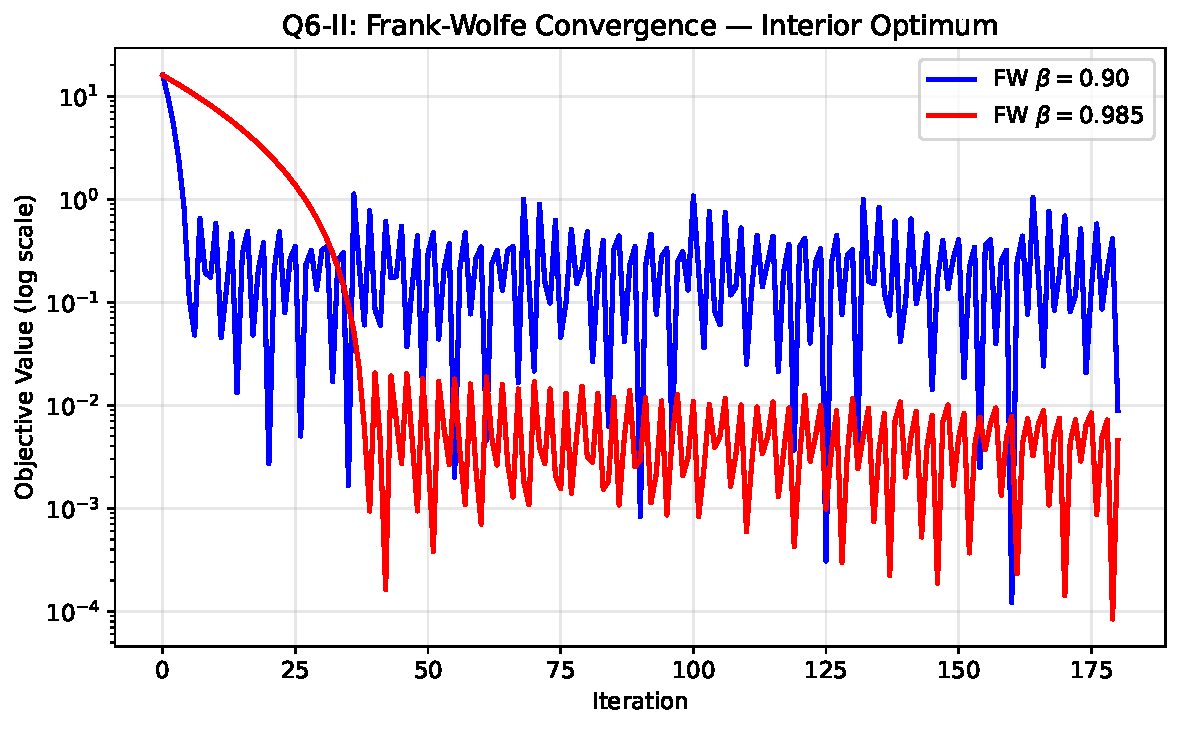
\includegraphics[width=0.85\textwidth]{figures/q6_fw_convergence.pdf}
\caption{Q6-II: Frank--Wolfe convergence for the interior optimum. With $\beta = 0.985$ (smaller steps), the final objective ($f = 0.0046$) is actually \emph{lower} than with $\beta = 0.90$ ($f = 0.0089$). This counterintuitive result occurs because larger steps ($\beta = 0.90$) cause greater oscillation as $z_k$ jumps between vertices of $\mathcal{X}$, while the conservative $\beta = 0.985$ allows smoother convergence with less oscillation.}
\label{fig:q6_fw_conv}
\end{figure}

\subsection{Boundary Optimum: $f(x) = x_1^2 + x_2^2$}

The unconstrained minimum $(0, 0)$ lies outside $\mathcal{X}$ (since $x_1 \geq 0.5$). The constrained minimum is at $(0.5, 0)$ on the boundary, with $f^{\star} = 0.25$.

\begin{figure}[H]
\centering
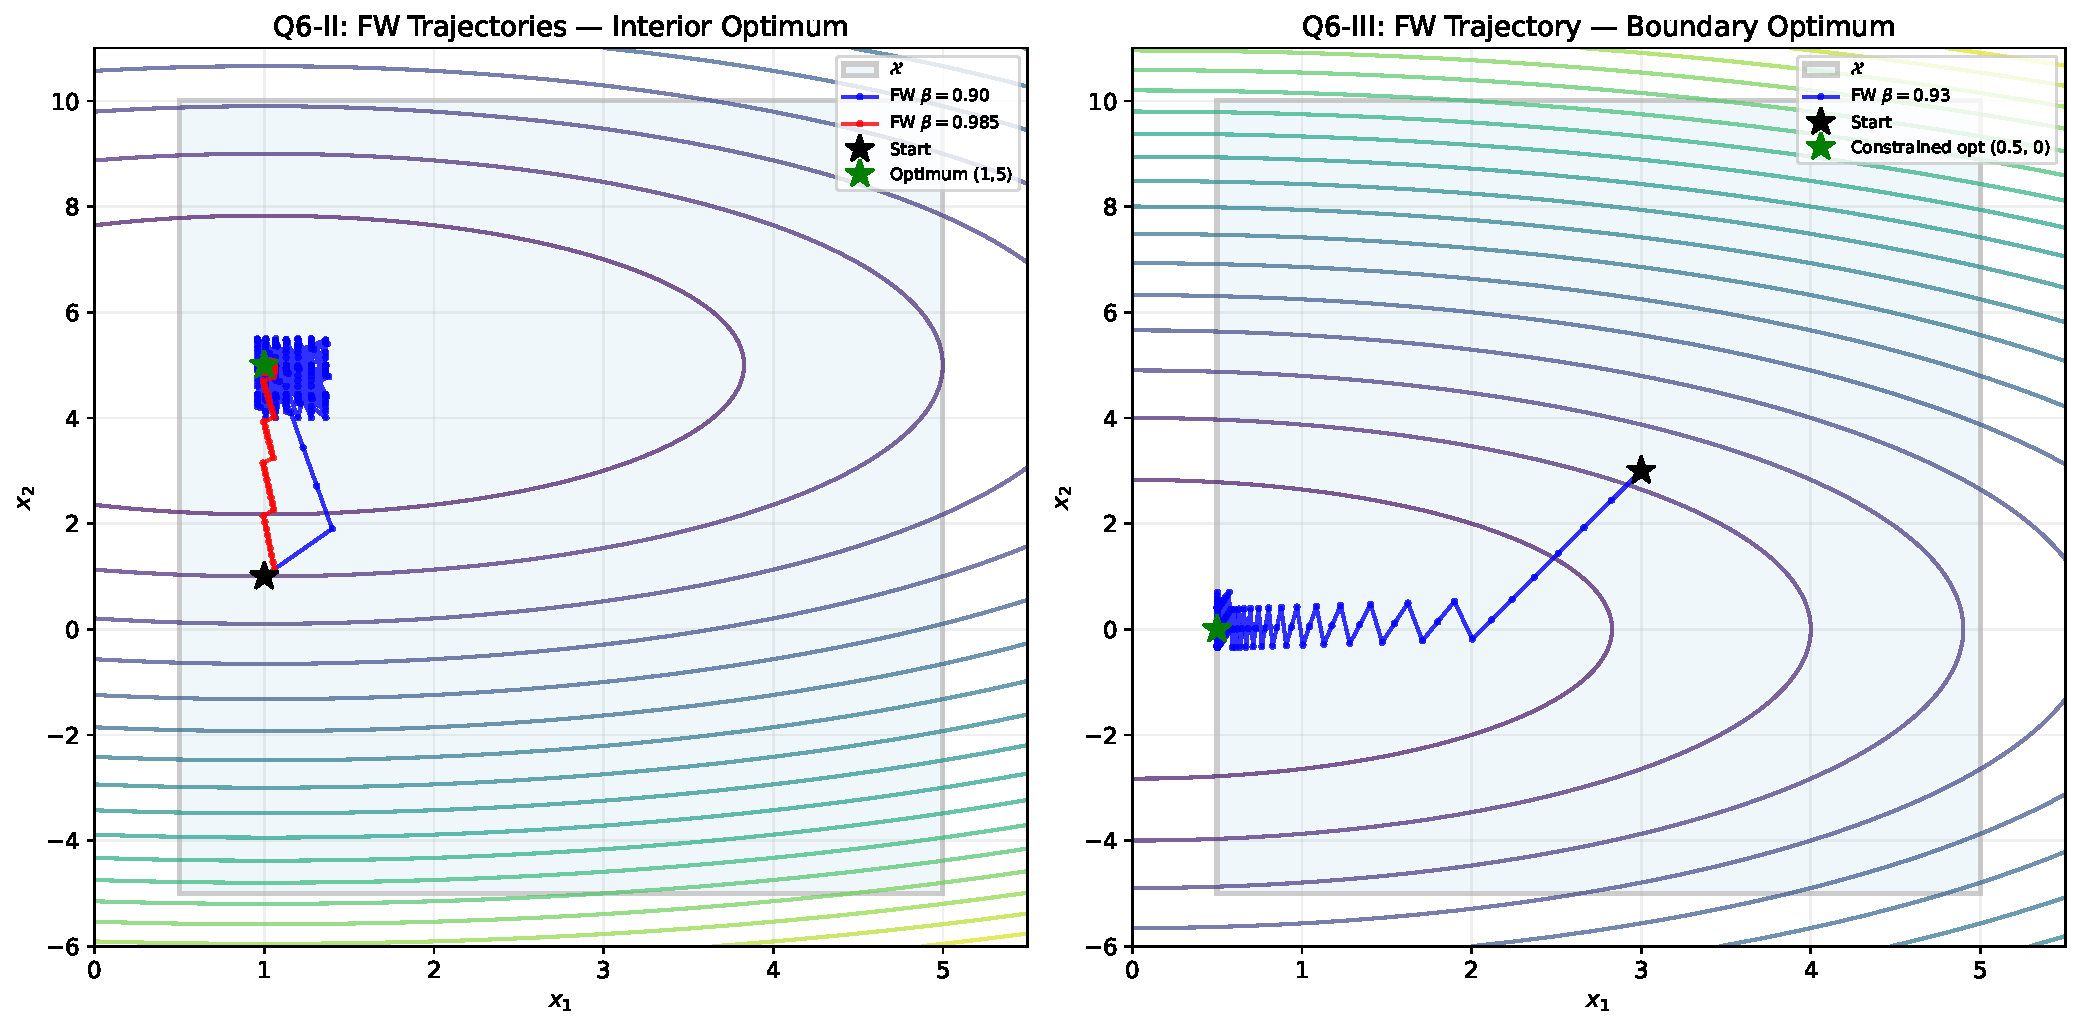
\includegraphics[width=\textwidth]{figures/q6_fw_contour.pdf}
\caption{Q6: Frank--Wolfe trajectories. Left: interior optimum --- trajectories converge towards $(1, 5)$ from $(1, 1)$. Right: boundary optimum --- trajectory converges towards $(0.5, 0)$ on the constraint boundary. Frank--Wolfe naturally handles constraints without explicit projection, since iterates are always convex combinations of feasible points.}
\label{fig:q6_fw_contour}
\end{figure}

\subsection{Evolution of $x_k$ and $z_k$}

\begin{figure}[H]
\centering
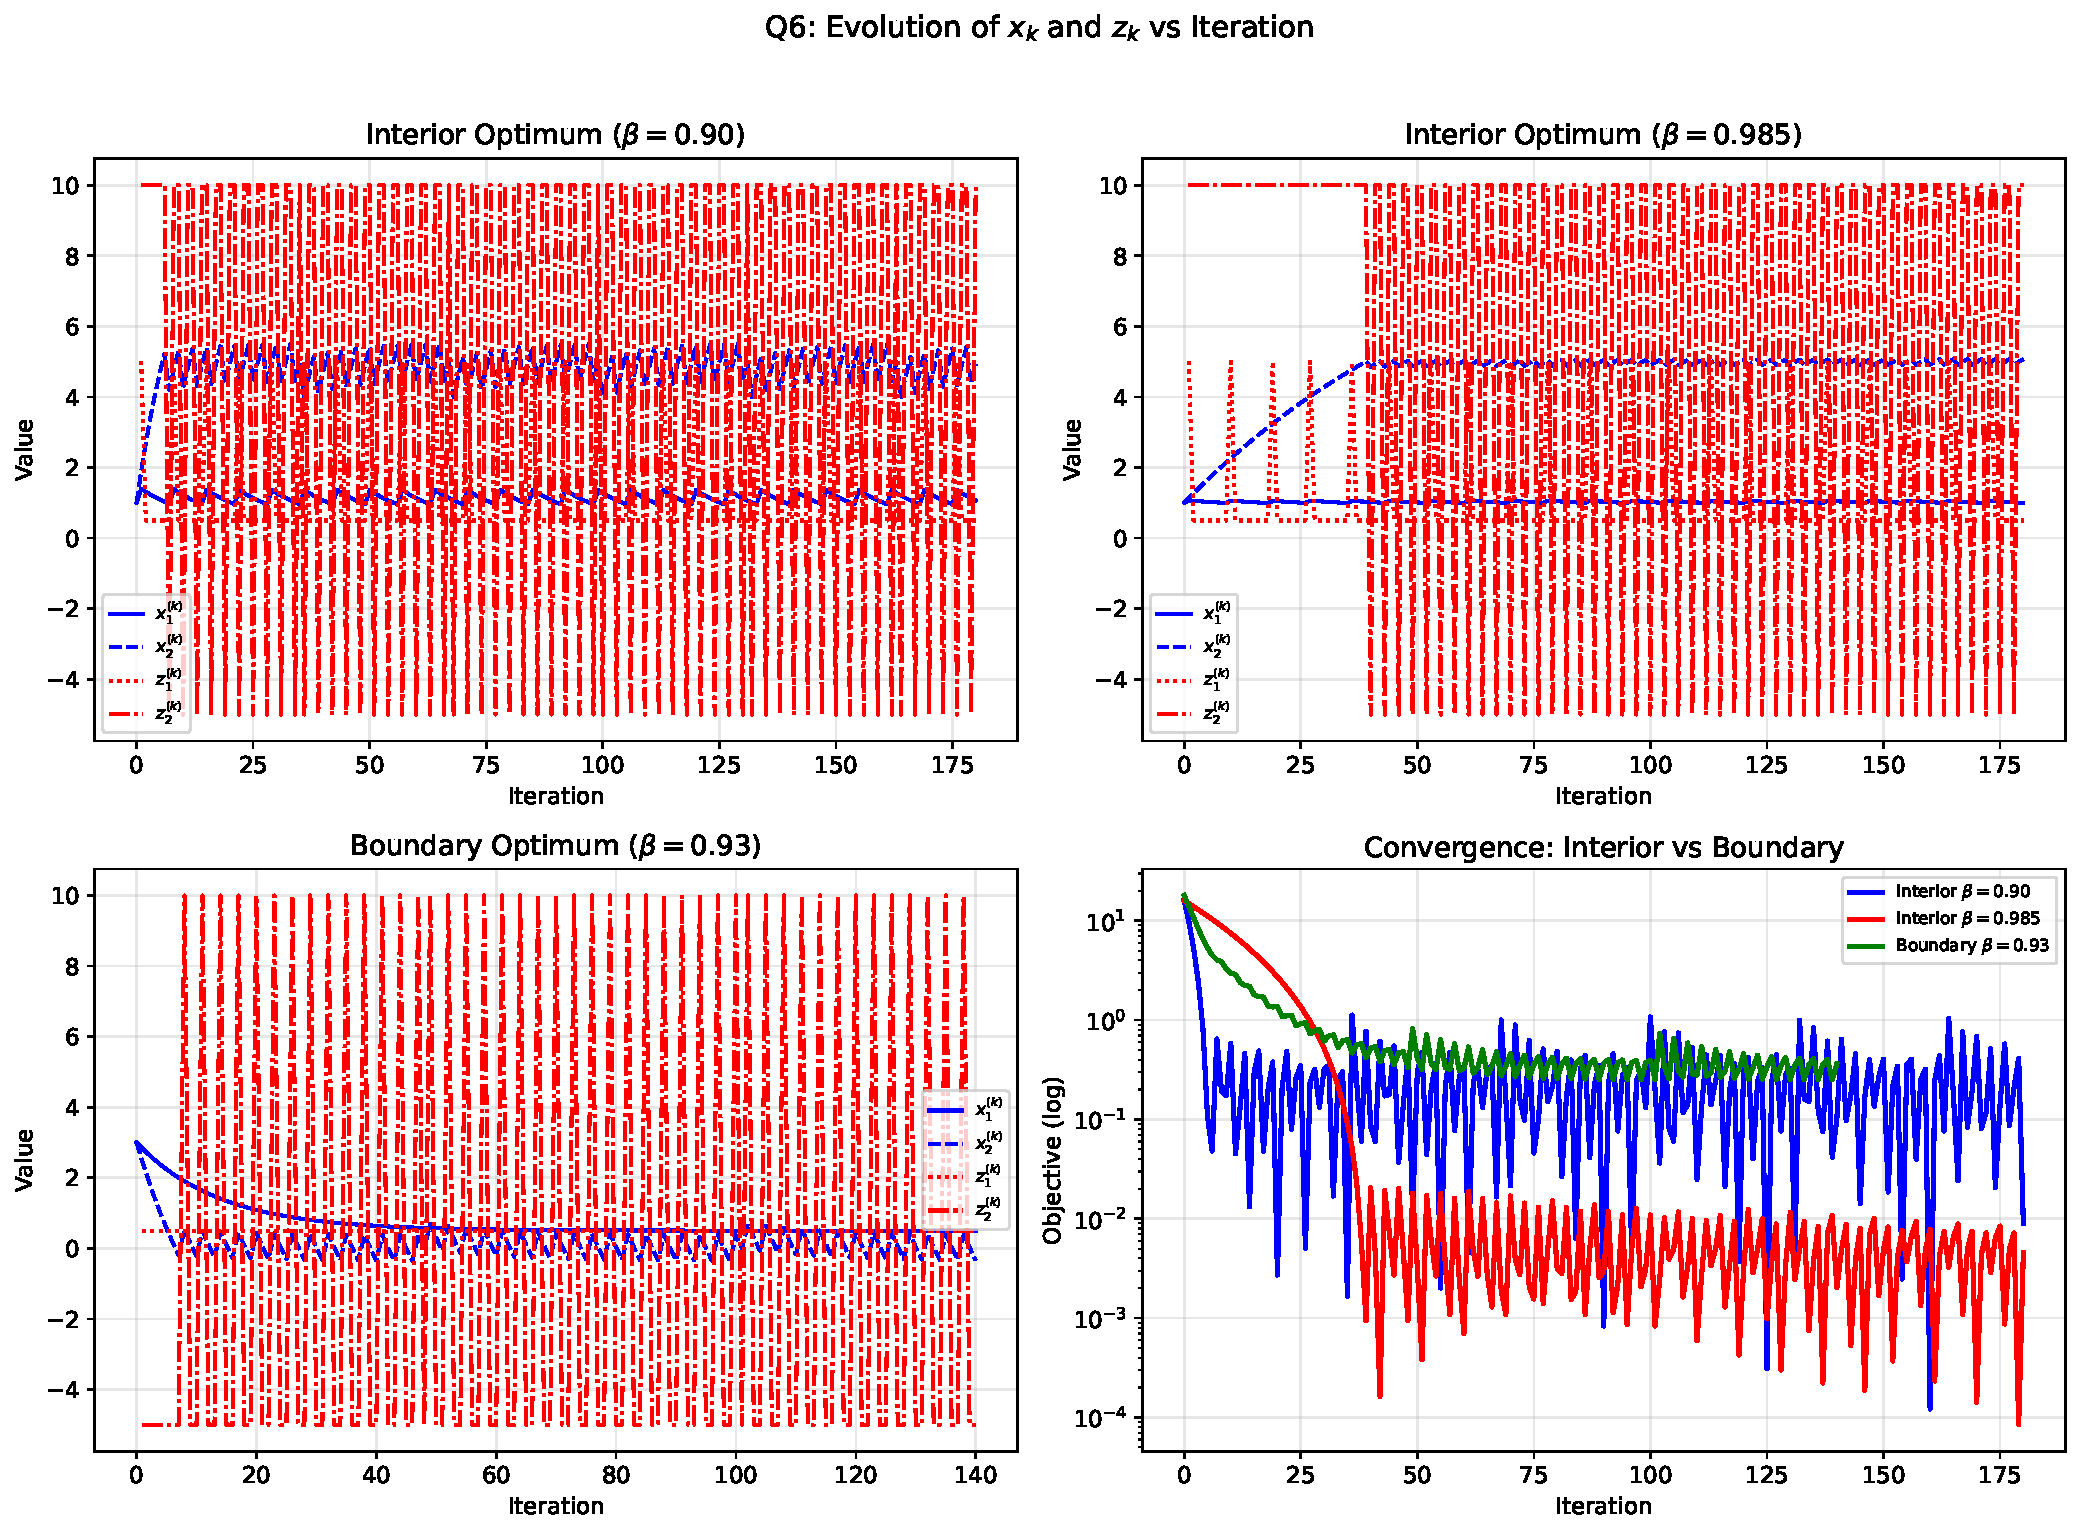
\includegraphics[width=\textwidth]{figures/q6_evolution.pdf}
\caption{Q6: Evolution of iterates and LP vertices. Top-left ($\beta = 0.90$): $x_k$ converges quickly but $z_k$ oscillates between vertices $(0.5, 10)$ and $(0.5, -5)$ as the gradient direction fluctuates. Top-right ($\beta = 0.985$): slower, smoother convergence. Bottom-left (boundary): $x_1$ converges to 0.5, $x_2$ towards 0. Bottom-right: convergence comparison --- boundary case converges to $f = 0.364$ after 140 iterations (above $f^{\star} = 0.25$, indicating more iterations are needed).}
\label{fig:q6_evolution}
\end{figure}

\begin{table}[H]
\centering
\caption{Q6: Final Frank--Wolfe positions and objective values.}
\label{tab:q6_final}
\begin{tabular}{lccc}
\toprule
\textbf{Case} & \textbf{Final $x$} & \textbf{$f(x)$} & \textbf{$f^{\star}$} \\
\midrule
Interior, $\beta = 0.90$ & $(1.066, 4.932)$ & 0.0089 & 0.0 \\
Interior, $\beta = 0.985$ & $(0.997, 5.067)$ & 0.0046 & 0.0 \\
Boundary, $\beta = 0.93$ & $(0.500, -0.337)$ & 0.3637 & 0.25 \\
\bottomrule
\end{tabular}
\end{table}

\subsection{Interior vs Boundary Behaviour}

\textbf{Interior optimum:} Frank--Wolfe converges but exhibits a characteristic ``zig-zag'' pattern. The LP vertex $z_k$ jumps between extreme points of $\mathcal{X}$ at each iteration, and the convex combination gradually averages these jumps. The general convergence rate is $O(1/k)$. Smaller $\beta$ (larger steps towards $z_k$) can be faster initially but introduces more oscillation near the optimum.

\textbf{Boundary optimum:} Frank--Wolfe is better suited to boundary optima because $z_k$ frequently selects the vertex closest to the constrained optimum. The iterate naturally approaches the boundary without needing explicit projection. However, the fixed $\beta$ schedule does not allow the step size to decay, resulting in residual oscillation. Using the standard $\gamma_k = 2/(k+2)$ schedule instead of fixed $\beta$ would improve convergence.

% ============================================================
\newpage
\appendix
\section{Python Code}
\label{app:code}
% ============================================================

The complete implementation is provided in the file \texttt{CS7DS2\_Final\_Code\_25336453.py}. Key algorithm implementations are reproduced below.

\begin{lstlisting}[caption={Gradient Descent}]
def gradient_descent(grad_fn, loss_fn, x0, alpha, n_iters):
    x = x0.copy().astype(float)
    x_hist, f_hist = [x.copy()], [loss_fn(x)]
    for _ in range(n_iters):
        x = x - alpha * grad_fn(x)
        x_hist.append(x.copy())
        f_hist.append(loss_fn(x))
    return np.array(x_hist), np.array(f_hist)
\end{lstlisting}

\begin{lstlisting}[caption={Polyak Step Size}]
def polyak_step(grad_fn, loss_fn, x0, f_star, eps, n_iters):
    x = x0.copy().astype(float)
    x_hist, f_hist, alpha_hist = [x.copy()], [loss_fn(x)], []
    for _ in range(n_iters):
        g = grad_fn(x)
        alpha_k = (loss_fn(x) - f_star) / (np.dot(g, g) + eps)
        alpha_hist.append(alpha_k)
        x = x - alpha_k * g
        x_hist.append(x.copy())
        f_hist.append(loss_fn(x))
    return np.array(x_hist), np.array(f_hist), np.array(alpha_hist)
\end{lstlisting}

\begin{lstlisting}[caption={Adagrad}]
def adagrad(grad_fn, loss_fn, x0, alpha0, eps, n_iters):
    x = x0.copy().astype(float)
    G = np.zeros_like(x)
    x_hist, f_hist, alpha_hist = [x.copy()], [loss_fn(x)], []
    for _ in range(n_iters):
        g = grad_fn(x)
        G += g**2
        eff_alpha = alpha0 / (np.sqrt(G) + eps)
        alpha_hist.append(np.mean(eff_alpha))
        x = x - eff_alpha * g
        x_hist.append(x.copy())
        f_hist.append(loss_fn(x))
    return np.array(x_hist), np.array(f_hist), np.array(alpha_hist)
\end{lstlisting}

\begin{lstlisting}[caption={RMSprop}]
def rmsprop(grad_fn, loss_fn, x0, alpha0, beta, eps, n_iters):
    x = x0.copy().astype(float)
    v = np.zeros_like(x)
    x_hist, f_hist, alpha_hist = [x.copy()], [loss_fn(x)], []
    for _ in range(n_iters):
        g = grad_fn(x)
        v = beta * v + (1 - beta) * g**2
        eff_alpha = alpha0 / (np.sqrt(v) + eps)
        alpha_hist.append(np.mean(eff_alpha))
        x = x - eff_alpha * g
        x_hist.append(x.copy())
        f_hist.append(loss_fn(x))
    return np.array(x_hist), np.array(f_hist), np.array(alpha_hist)
\end{lstlisting}

\begin{lstlisting}[caption={Heavy Ball / Polyak Momentum}]
def heavy_ball(grad_fn, loss_fn, x0, alpha, beta, n_iters):
    x = x0.copy().astype(float)
    z = np.zeros_like(x)
    x_hist, f_hist = [x.copy()], [loss_fn(x)]
    for _ in range(n_iters):
        g = grad_fn(x)
        z = beta * z + alpha * g
        x = x - z
        x_hist.append(x.copy())
        f_hist.append(loss_fn(x))
    return np.array(x_hist), np.array(f_hist)
\end{lstlisting}

\begin{lstlisting}[caption={Nesterov Momentum}]
def nesterov_momentum(grad_fn, loss_fn, x0, alpha, beta_max, n_iters):
    x = x0.copy().astype(float)
    z = np.zeros_like(x)
    x_hist, f_hist = [x.copy()], [loss_fn(x)]
    for k in range(1, n_iters + 1):
        beta_k = min((k - 1) / (k + 2), beta_max)
        lookahead = x + beta_k * z
        g = grad_fn(lookahead)
        z = beta_k * z - alpha * g
        x = x + z
        x_hist.append(x.copy())
        f_hist.append(loss_fn(x))
    return np.array(x_hist), np.array(f_hist)
\end{lstlisting}

\begin{lstlisting}[caption={Adam Optimiser}]
def adam_optimiser(grad_fn, loss_fn, x0, alpha, beta1, beta2, eps, n_iters):
    x = x0.copy().astype(float)
    m_vec, v_vec = np.zeros_like(x), np.zeros_like(x)
    x_hist, f_hist = [x.copy()], [loss_fn(x)]
    for t in range(1, n_iters + 1):
        g = grad_fn(x)
        m_vec = beta1 * m_vec + (1 - beta1) * g
        v_vec = beta2 * v_vec + (1 - beta2) * g**2
        m_hat = m_vec / (1 - beta1**t)
        v_hat = v_vec / (1 - beta2**t)
        x = x - alpha * m_hat / (np.sqrt(v_hat) + eps)
        x_hist.append(x.copy())
        f_hist.append(loss_fn(x))
    return np.array(x_hist), np.array(f_hist)
\end{lstlisting}

\begin{lstlisting}[caption={Newton's Method}]
def newtons_method(grad_fn, hess_fn, loss_fn, x0, alpha, n_iters, damping=1e-8):
    x = x0.copy().astype(float)
    x_hist, f_hist, update_norms = [x.copy()], [loss_fn(x)], []
    for _ in range(n_iters):
        g = grad_fn(x)
        H = hess_fn(x) if callable(hess_fn) else hess_fn
        H_reg = H + damping * np.eye(len(x))
        try:
            p = np.linalg.solve(H_reg, g)
        except np.linalg.LinAlgError:
            p = g
        update_norms.append(np.linalg.norm(alpha * p))
        x = x - alpha * p
        x_hist.append(x.copy())
        f_hist.append(loss_fn(x))
    return np.array(x_hist), np.array(f_hist), np.array(update_norms)
\end{lstlisting}

\begin{lstlisting}[caption={Nelder--Mead Simplex}]
def nelder_mead(loss_fn, x0, step, n_iters, alpha_r=1.0, gamma=2.0, rho=0.5, sigma=0.5):
    n = len(x0)
    simplex = np.zeros((n + 1, n))
    simplex[0] = x0.copy()
    for i in range(n):
        simplex[i + 1] = x0.copy()
        simplex[i + 1][i] += step
    f_vals = np.array([loss_fn(v) for v in simplex])
    centroid_hist = [np.mean(simplex, axis=0).copy()]
    f_best_hist = [np.min(f_vals)]
    for _ in range(n_iters):
        order = np.argsort(f_vals)
        simplex = simplex[order]; f_vals = f_vals[order]
        centroid = np.mean(simplex[:-1], axis=0)
        x_r = centroid + alpha_r * (centroid - simplex[-1])
        f_r = loss_fn(x_r)
        if f_vals[0] <= f_r < f_vals[-2]:
            simplex[-1] = x_r; f_vals[-1] = f_r
        elif f_r < f_vals[0]:
            x_e = centroid + gamma * (centroid - simplex[-1])
            f_e = loss_fn(x_e)
            if f_e < f_r: simplex[-1] = x_e; f_vals[-1] = f_e
            else: simplex[-1] = x_r; f_vals[-1] = f_r
        else:
            if f_r < f_vals[-1]:
                x_c = centroid + rho * (x_r - centroid)
                f_c = loss_fn(x_c)
                if f_c <= f_r: simplex[-1] = x_c; f_vals[-1] = f_c
                else:
                    for i in range(1, n+1):
                        simplex[i] = simplex[0]+sigma*(simplex[i]-simplex[0])
                        f_vals[i] = loss_fn(simplex[i])
            else:
                x_c = centroid + rho * (simplex[-1] - centroid)
                f_c = loss_fn(x_c)
                if f_c < f_vals[-1]: simplex[-1] = x_c; f_vals[-1] = f_c
                else:
                    for i in range(1, n+1):
                        simplex[i] = simplex[0]+sigma*(simplex[i]-simplex[0])
                        f_vals[i] = loss_fn(simplex[i])
        centroid_hist.append(np.mean(simplex, axis=0).copy())
        f_best_hist.append(np.min(f_vals))
    return np.array(centroid_hist), np.array(f_best_hist), simplex
\end{lstlisting}

\begin{lstlisting}[caption={Frank--Wolfe Algorithm}]
def frank_wolfe(grad_fn, loss_fn, x0, bounds, beta, n_iters):
    x = x0.copy().astype(float)
    x_hist, f_hist, z_hist = [x.copy()], [loss_fn(x)], []
    for _ in range(n_iters):
        g = grad_fn(x)
        z = np.array([bounds[i][0] if g[i] > 0 else bounds[i][1]
                       for i in range(len(g))])
        z_hist.append(z.copy())
        x = beta * x + (1 - beta) * z
        x_hist.append(x.copy())
        f_hist.append(loss_fn(x))
    return np.array(x_hist), np.array(f_hist), np.array(z_hist)
\end{lstlisting}

\end{document}
